%% Latex template for PhD dissertation or MS thesis
%% Electrical and Computer Engineering Department
%% Brigham Young University
%% Last Modified:  March 2012

\documentclass[12pt]{report}

%%%%%%%%%%%%%%%%%%%%%%%%%%%%%%%%%%%%%%%%%%%%%%%%%%%%%%%%
%  Setup BYU thesis format
%%%%%%%%%%%%%%%%%%%%%%%%%%%%%%%%%%%%%%%%%%%%%%%%%%%%%%%%
\usepackage{amsmath}
\interdisplaylinepenalty=2500
\usepackage{cite}
\usepackage{dcolumn}
\usepackage{times}
\usepackage{fancyhdr}
\usepackage{setspace}

\usepackage{latexsym} % Need this for \Box
\usepackage{graphicx}
%\usepackage[pdftex]{graphicx}
\usepackage{epstopdf}

\usepackage{byustyle}
\usepackage{epstopdf}
\usepackage{booktabs}
\usepackage{nicefrac}
\usepackage{mathtools}
% Setup the byu style sheet
\byustylesetup{%
    %
    %isdissertation = true,            % Uncomment this if you're doing a PhD dissertation
    %etdsubmission = true,            % Uncomment this if you're compiling it for ETD submission
    singlepageabstract = true, % Comment this out if your abstract is multiple pages
    singlepageacknowledgements = true, % Uncomment this if your Acknowledgements is multiple pages
    %
    % Definitions of names needed in thesis/dissertation
    deptname          = Department of Electrical and Computer Engineering,    %
    collegename       = Ira A. Fulton College of\\Engineering and Technology, %
    committeechairman = Michael D. Rice,                      %
    committeemembera  = Brian D. Jeffs,                         %
    committeememberb  = Brian A. Mazzeo,                          %
    %committeememberc  = Firstname Mi. Lastname,                    % PhD Only
    %committeememberd  = Firstname Mi. Lastname,                     % PhD Only
    graddate = April 2017,  % Leave commented for current month and year
    %copyrightyear = 2012,      % Leave commented for current year
    % uncomment the keywords for a dissertation
    %keywords         = {elecromagnetic waves, crazy circuits}
    %
    % Uncomment to shorten for proofreading purposes
    %noabstract = true,         % Don't show the abstract page
    %nouniversitypages = true,  % Don't show any of the "university pages"
    %noacknowledgements = true, % Don't show the Acknowledgements page
    %notableofcontents = true,  % Don't show the Table of Contents
    %nolistoffigures = true,    % Don't show the List of Figures
    %nolistoftables = true,     % Don't show the List of Tables
    %notocandlists = true,      % Don't show the Table of Contents, List of Figures, or the List of Tables
    %noheaderatall = true,      % Don't show any of the BYU Thesis header pages
}
%%%%%%%%%%%%%%%%%%%%%%%%%%%%%%%%%%%%%%%%%%%%%%%%%%%%%%%%
%  END:  Setup BYU thesis format
%%%%%%%%%%%%%%%%%%%%%%%%%%%%%%%%%%%%%%%%%%%%%%%%%%%%%%%%%

%%%%%%%%%%%%%%%%%%%%%%%%%%%%%%%%%%%%%%%%%%%%%%%%%%%%%%%%
%  Include other \usepackage{} statements here.
%    Add one package at a time.
%    Warning:  Some packages are not compatible with byuthesis.sty
%%%%%%%%%%%%%%%%%%%%%%%%%%%%%%%%%%%%%%%%%%%%%%%%%%%%%%%%%
%\usepackage[normalmargins]{savetrees} % prints smaller to save trees (draft only)
\usepackage{amsmath,amssymb} % math definitions
\usepackage{graphicx}        % for figures
\usepackage{subfigure}       % for figures with multiple subfigures
\usepackage{setspace}        % so all the captions will be single spaced
%%%%%%%%%%%%%%%%%%%%%%%%%%%%%%%%%%%%%%%%%%%%%%%%%%%%%%%%
%  END: Include other \usepackage{} statements here.
%%%%%%%%%%%%%%%%%%%%%%%%%%%%%%%%%%%%%%%%%%%%%%%%%%%%%%%%%

%%%%%%%%%%%%%%%%%%%%%%%%%%%%%%%%%%%%%%%%%%%%%%%%%%%%%%%%
% For doing bookmarks in the PDF file
%%%%%%%%%%%%%%%%%%%%%%%%%%%%%%%%%%%%%%%%%%%%%%%%%%%%%%%%%
% For more info, see:
% http://www.geocities.com/kijoo2000/latex2pdf.pdf
% http://www.tug.org/applications/hyperref/manual.html
\usepackage[driverfallback=dvipdfm,backref,pagebackref,plainpages=false]{hyperref}
\hypersetup{
    %bookmarks    = true, % Make bookmarks (default=true). This option
                          %cannot be used after package has been loaded,
                          %thus use like this: \usepackage[bookmarks=false]{hyperref}.
    %
    breaklinks   = false, % Allow link text to break across lines (default=false).
    linktocpage  = false, % make page number, not text, be link on TOC, LOF and LOT
    colorlinks   = false, % Color the text of links (true) or put color frames over
                          % the links (false).
% NOTE: if you need to use a dvi->ps->pdf path for things like PSTricks, you
% may find that commenting out the next line is necessary.
    %pdfborder    = 001,   % sets the default for pdf links                      
    pdfstartview = {FitH}, % Set the startup page view. Possible options are:
                           % FitH: Fit whole width of page
                           % FitV: Fit whole height of page
                           % FitB: Fit whole “Bounding Box” page
                           % FitBH: Fit whole width of “Bounding Box” of page
                           % FitBV: Fit whole height of “Bounding Box” of page
    bookmarksnumbered  = true, % Put section numbers in bookmarks (default=false)
    bookmarksopen      = true, % Open up the bookmark trees (default=false).
    bookmarksopenlevel = 1, % Level to which bookmarks are open (default=\maxdimen).
    bookmarkstype      = toc, % Specify which toc file to mimic (default=toc).
    pdfpagemode        = {UseOutlines}, %  Specify how document starts when opened ({None}).
                                        % Possible options are:,
                                        % None: Neither bookmarks nor thumbnails are visible.
                                        % UseOutlines: Bookmarks are visible.
                                        % UseThumbs: Thumbnails are visible.
                                        % FullScreen: Full-screen mode
    pdftitle    = {JeffRavertMastersThesis},
    pdfauthor   = {Jeff Ravert},
    pdfcreator  = {Jeff Ravert},
    pdfsubject  = {Jeff Ravert's Master's Thesis},
    pdfkeywords = {GPU, Equalizer, Estimator, FPGA, BYU},
}
%%%%%%%%%%%%%%%%%%%%%%%%%%%%%%%%%%%%%%%%%%%%%%%%%%%%%%%%
%  END: For doing bookmarks in the PDF file
%%%%%%%%%%%%%%%%%%%%%%%%%%%%%%%%%%%%%%%%%%%%%%%%%%%%%%%%%

%%%%%%%%%%%%%%%%%%%%%%%%%%%%%%%%%%%%%%%%%%%%%%%%%%%%%%%%
%                Macros
%  Define macros here
%%%%%%%%%%%%%%%%%%%%%%%%%%%%%%%%%%%%%%%%%%%%%%%%%%%%%%%%%
\def\proof{\noindent{\it Proof: }}
\def\QED{\mbox{\rule[0pt]{1.5ex}{1.5ex}}}
\def\endproof{\hspace*{\fill}~\QED\par\endtrivlist\unskip}
%
\newcommand{\norm}[1]{\left\|#1\right\|}
\newcommand{\abs}[1]{\left|#1\right|}
\newcommand{\defeq}{\stackrel{\triangle}{=}}
\newcommand{\re}{\mathbb{R}} % real numbers
\newcommand{\OMIT}[1]{{}} % omit sections of text
\newcommand{\pd}[2]{\ensuremath{\frac{\partial #1}{\partial #2}}} % partial derivative

%%%%%%%%%%%%%%%%%%%%%%%%%%%%%%%%%%%%%%%%%%%%%%%%%%%%%%%%%
%                End Macros
%%%%%%%%%%%%%%%%%%%%%%%%%%%%%%%%%%%%%%%%%%%%%%%%%%%%%%%%%

% To only print a few chapters without changing the reference numbers,
% uncomment the chapters you want
%\includeonly{intro}
%\includeonly{chapter2}
%\includeonly{appendixa}

%%%%%%%%%%%%%%%%%%%%%%%%%%%%%%%%%%%%%%%%%%%%%%%%%%%%%%%%%
% Start Document
%%%%%%%%%%%%%%%%%%%%%%%%%%%%%%%%%%%%%%%%%%%%%%%%%%%%%%%%%

\begin{document}

% Define Title & Author
\title{GPU Implementation of Data-Aided Equalizers}
\author{Jeffrey T. Ravert}

% For displaying the BYU Thesis header
% This command assumes that there are documents called abstract.tex and
% acknowledgements.tex that will be included in the header
\showBYUHeader


% Include chapters of the thesis here:
% each chapter should be in a file with a .tex extension and the text
% of the file should begin with \chapter{Chapter Title}, followed
% by the text of the chapter.
%  Note: the introduction is considered Chapter 1.
%\chapter{Introduction}
This is an example of the introduction. It's pretty simple and shows off
some of the basic commands.

\section{First Section}
This part shows how you can divide things into sections.

\subsection{First Subsection}
Also into subsections.

\subsubsection{First Subsubsection}
And even Subsubsections but they don't work correctly with Chapters and so I
would recommend against using them.

\subsection{Second Subsection}
Which really helps organization and automatically gets added to the Table
of Contents and gets linked to by the hyperref package.

\section{Citation Example}
One of the coolest part about \LaTeX\ is BibTeX. You can just call
the $\backslash$cite command and it will do all of the bibliography
stuff for you as long as there is an entry in the refs.bib file.
Here's an example of citing previous works
\cite{SomeSweetBook06,SomeSweetArticle06}.

\section{Math and Equation Example}
Here's how to use inline math mode to define lambda like this,
$\lambda$, and how to declare Equations~\eqref{eqn:definition_Ix}
and~\eqref{eqn:definition_Iy}

\begin{equation} \label{eqn:definition_Ix}
I_x(x,y) = \pd{I(x,y)}{x},
\end{equation}

\begin{equation}\label{eqn:definition_Iy}
I_y(x,y) = \pd{I(x,y)}{y}.
\end{equation}

If you don't want equation numbers, use
\[
\text{sign}(x) = \begin{cases}
                 1,  &\quad x> 0 \\
                 -1, &\quad x<0 \\
                 0,  &\quad \text{otherwise}
                 \end{cases}.
\]


 Or you can create equation arrays like
\begin{align}
  \alpha &= \beta^\gamma \notag \\
  x &= \frac{1}{\alpha} \label{eq:cool_1} \\
  y &= \sqrt{\abs{\frac{\gamma}{\beta}}} \notag \\
  \zeta &= x^y \label{eq:cool_2}.
\end{align}


The lines in the array can be referenced by saying things like: In
Eq.~\eqref{eq:cool_1} we show a cool equation, but its not nearly as
cool as Eq.~\eqref{eq:cool_2}.

\section{Fixed Width Figure Example} \label{sec:intro_figure_example}
This part also shows how to include a basic figure like the one
shown in Figure~\ref{fig:intro_stuff}

\begin{figure}[hhhhhtb]
  \centering
  
\includegraphics[width=5.5in]{figures/intro/stuff}
  \caption[Example Fixed Width Figure]{
This figure is just a simple figure with a width set at 5.5in. An example of a
figure whose size depends on the width of the page is given in
Figure \ref{fig:appendix_some_pic} in Section \ref{sec:appendxia_figure_example}}
%
  \label{fig:intro_stuff}
\end{figure}

\section{All Done}
You know have seen a lot of the basics and now you can see some
other fancy stuff in Chapter~\ref{chp:chapter2}.

%\chapter{Making Tables}
\label{chp:chapter2}
\graphicspath{{figures/}{figures/chapter2/}}

\section{Making a Table}
An example \LaTeX\ table is shown below in Table~\ref{tab:comparison}.
You make a table by starting a table environment with a caption
and label.  You can specify the text that shows up in the Table of
Contents using the optional parameter box, [], that's at the
beginning of the $\backslash$caption command. You tell the table how
many columns in the beginning of the tabular environment using a
command like this: $|$ l $|$ c $|$ r $|$. That would create a table with 3 columns
that are left-aligned, centered and right-aligned, in that order. The $|$'s tell \LaTeX\ that
you want bars separating the columns. Of course, you can also make tables without the $|$ characters, in which case no lines will be added between the fields, which often looks better. You can also add horizontal
lines using the $\backslash$hline command. This example is also centered in the page using the
$\backslash$centering command.
%
\begin{table}[b]
\centering
\savebox{\tempbox}{
%
\begin{tabular}{|l|c|c|r|}
\hline

Table Name  & Column 2 & Column 3   & Column 4 \\
\hline
First Row   & 4780286  & 72.941376  & A \\
Second Row  & 4069335  & 62.093124  & B \\
Third Row   & 4074900  & 62.178040  & C \\
\hline
Fourth Row  & 4000000  & 60.000000  & Z \\
\hline

\end{tabular}}
% set width
\ifdim\wd\tempbox<\TPTminimum\relax \tempwidth=\TPTminimum\relax
\else\tempwidth=\wd\tempbox
\fi
% format
\begin{minipage}{\tempwidth}\centering
\caption[Example table]{Description of the table, where the caption is long enough to go onto more than one line. The table caption should not extend beyond the edges of the table, and should make an ``inverted pyramid.''}
\label{tab:comparison}
\usebox{\tempbox}
%\end{threeparttable}
\end{minipage}
\end{table}
%

Landscape tables can also be inserted, if desired, using the \verb-sidewaystable- environment, which is defined in the \verb!rotating! package. An example is found on the next page, in Table~\ref{tab:landscape}. Note that landscape tables and figures should be the exception rather than the rule, since they are more awkward to read. However, if you have an especially wide table or figure that cannot be reduced in size without losing required resolution, placing it in landscape may be a good idea.
\begin{sidewaystable}
\centering
\savebox{\tempbox}{
\setlength{\tabcolsep}{6mm}
\begin{tabular}{lcccc}
Year & Method of CVD Deposition & Thickness ($\mu$m) & Hardness (MPa) & Resistivity ($\Omega\cdot$m)\\ 
\hline\\[-11pt]
1999 & LPCVD & 5.1 & 175 & 2.3$\times10^{-5}$\\
2000 & PECVD & 17.2 & 101& 1.5$\times10^{-5}$\\
2002 & PECVD & 4.3 & 55 & 3.4$\times10^{-5}$\\
2004 & LPCVD & 1.1 & 225 & 5.1$\times10^{-5}$\\
\hline
\end{tabular}}
% set width
\ifdim\wd\tempbox<\TPTminimum\relax \tempwidth=\TPTminimum\relax
\else\tempwidth=\wd\tempbox
\fi
% format
\begin{minipage}{\tempwidth}\centering
\caption{A landscape table}\vspace*{6pt}
\label{tab:landscape}
\usebox{\tempbox}
%\end{threeparttable}
\end{minipage}
\end{sidewaystable}
%%%%%%%%%%%%%%%%%%%%%%%%%%%%%%%%%%%%%%%%%%%%%%%%%%%%%%%%%%%%%%%%%%%%%%%%%%%%%%%%%%%%%%%%%%%%%%%
%%%%%%%%%%%%%%%%%%%%%%%%%%%%%%%%%%%%%%%%%%%%%%%%%%%%%%%%%%%%%%%%%%%%%%%%%%%%%%%%%%%%%%%%%%%%%%
%%%%%%%%%%% GPU
%%%%%%%%%%%%%%%%%%%%%%%%%%%%%%%%%%%%%%%%%%%%%%%%%%%%%%%%%%%%%%%%%%%%%%%%%%%%%%%%%%%%%%%%%%%%%%
%%%%%%%%%%%%%%%%%%%%%%%%%%%%%%%%%%%%%%%%%%%%%%%%%%%%%%%%%%%%%%%%%%%%%%%%%%%%%%%%%%%%%%%%%%%%%%


% \cleardoublepage
\chapter{Signal Processing with GPUs}
\label{sec:gpu}

%\section{Overview}
%
%A Graphics Processing Unit (GPU) is a computational unit with a specialized, highly-parallel architecture well-suited to processing large blocks of data.
%The performance advantage derives from the GPUs ability to perform a large number of parallel computations on the large data block.
%Historically, the large block of data was graphics data and the computations were limited to those required for graphics operations.
%Since about 2006, there has been increasing interest in using genral purpose GPUs for more general processing tasks such as machine learning, oil exploration, scientific image processing, linear algebra, statistics, and 3D reconstruction \cite{wikipedia-gpu:2015}.
%This project leverages this trend and applies GPU processing to the estimation, computation, and filtering operations required for data-aided equalization.
%
%Typically, the GPU architecture comprises a large memory block accessible by several (up to a few thousand) processing units simultaneously.
%For example, memory and processing units (called ``CUDA cores'') for the two Nvidia GPUs used in this project are summarized in Table~\ref{tab:gpu-resources}.
%Consequently, algorithms that are highly parallel are best suited for the GPU.
%In constrast, sequential algorithms (e.g., a phase lock loop!) are not well suited for the GPU.
%
%Programming the Nvidia GPUs is written in the C++ computer language with API extensions known as CUDA (Compute Unified Device Architecture).
%The CUDA API is ``a software layer that gives direct access to the GPU's virtual instruction set and parallel computational elements'' \cite{wikipedia-cuda:2015}.
%CUDA allows the C++ program, running on the host CPU, to launch special functions---known as kernels--- on the GPU while allowing some of the functionality to remain on the host CPU.
%
%The choice to use GPUs, rather than FPGAs, for this project include the following:
%\begin{enumerate}
%	\item The desire to test the performance of four equalizers operating in parallel on the
%		received data is a good match to GPU structure.
%	\item Programming in C++ has advantages over VHDL designs in an FPGA.
%		Development time is much shorter and debugging is quite a bit easier.
%		Small modifications are much easier with C++ and GPUs than with VHDL in and FPGA.
%	\item  Because the GPU supports floating point operations, the complications of tracking
%		``digit growth'' in fixed-point operations (on an FPGA) are eliminated.
%\end{enumerate}
%GPUs are unlikely to be used for telemetry demodulators in the foreseeable future.
%However, because the point of the project is to assess the performance of competing algorithms,
%this fact is less important.
%Once identified, the ``best'' equalizer algorithm can be designed in VHDL and incorporated
%into the FPGA-based demodulators commonly found on the telemetry market.
%
%The unique features of the GPU architecture require the designer to rethink how the
%signal processing is organized.
%DRAM memory limitations on the FPGA limit the number of samples per transfer $39{,}321{,}600$
%complex-valued samples ($314{,}572{,}800$ Bytes).
%This data, corresponding to $3{,}103$ packets,
%is loaded into the GPU memory (cf. Table~\ref{tab:gpu-resources}).
%Here starting indexes of the $3{,}103$ occurrences of the preamble are found.
%Subsequent signal processing for each packet is performed \textit{in parallel}.
%In the end, $3{,}103 \times 6{,}144 = 19{,}064{,}832$ data bits \textit{per equalizer}
%are produced at the end of the processing applied to each block.
%A conceptual block diagram of this organization is illustrated in Figure~\ref{fig:signal-flow-gpu}.
%The preamble detector (or frame synchronizer), frequency offset estimator, channel estimator, and
%noise variance estimator are described in Section~\ref{sec:estimators}.
%The equalizers are described in Section~\ref{sec:eq}.
%
%
%\begin{table}
%\caption{The computational resources available with three Nvidia GPUs used in this project (1x Tesla k40 2x Tesla K20).}
%\label{tab:gpu-resources}
%\begin{center}
%\begin{tabular}{lll}
%	\toprule
%	Feature & Tesla k40 & Tesla K20 \\ \midrule
%	Memory size (GDDR5) & 12 GB & 5 GB \\
%	CUDA cores & 2880 & 2496 \\ \bottomrule
%\end{tabular}
%\end{center}
%\end{table}
%
%\begin{figure}
%	\centering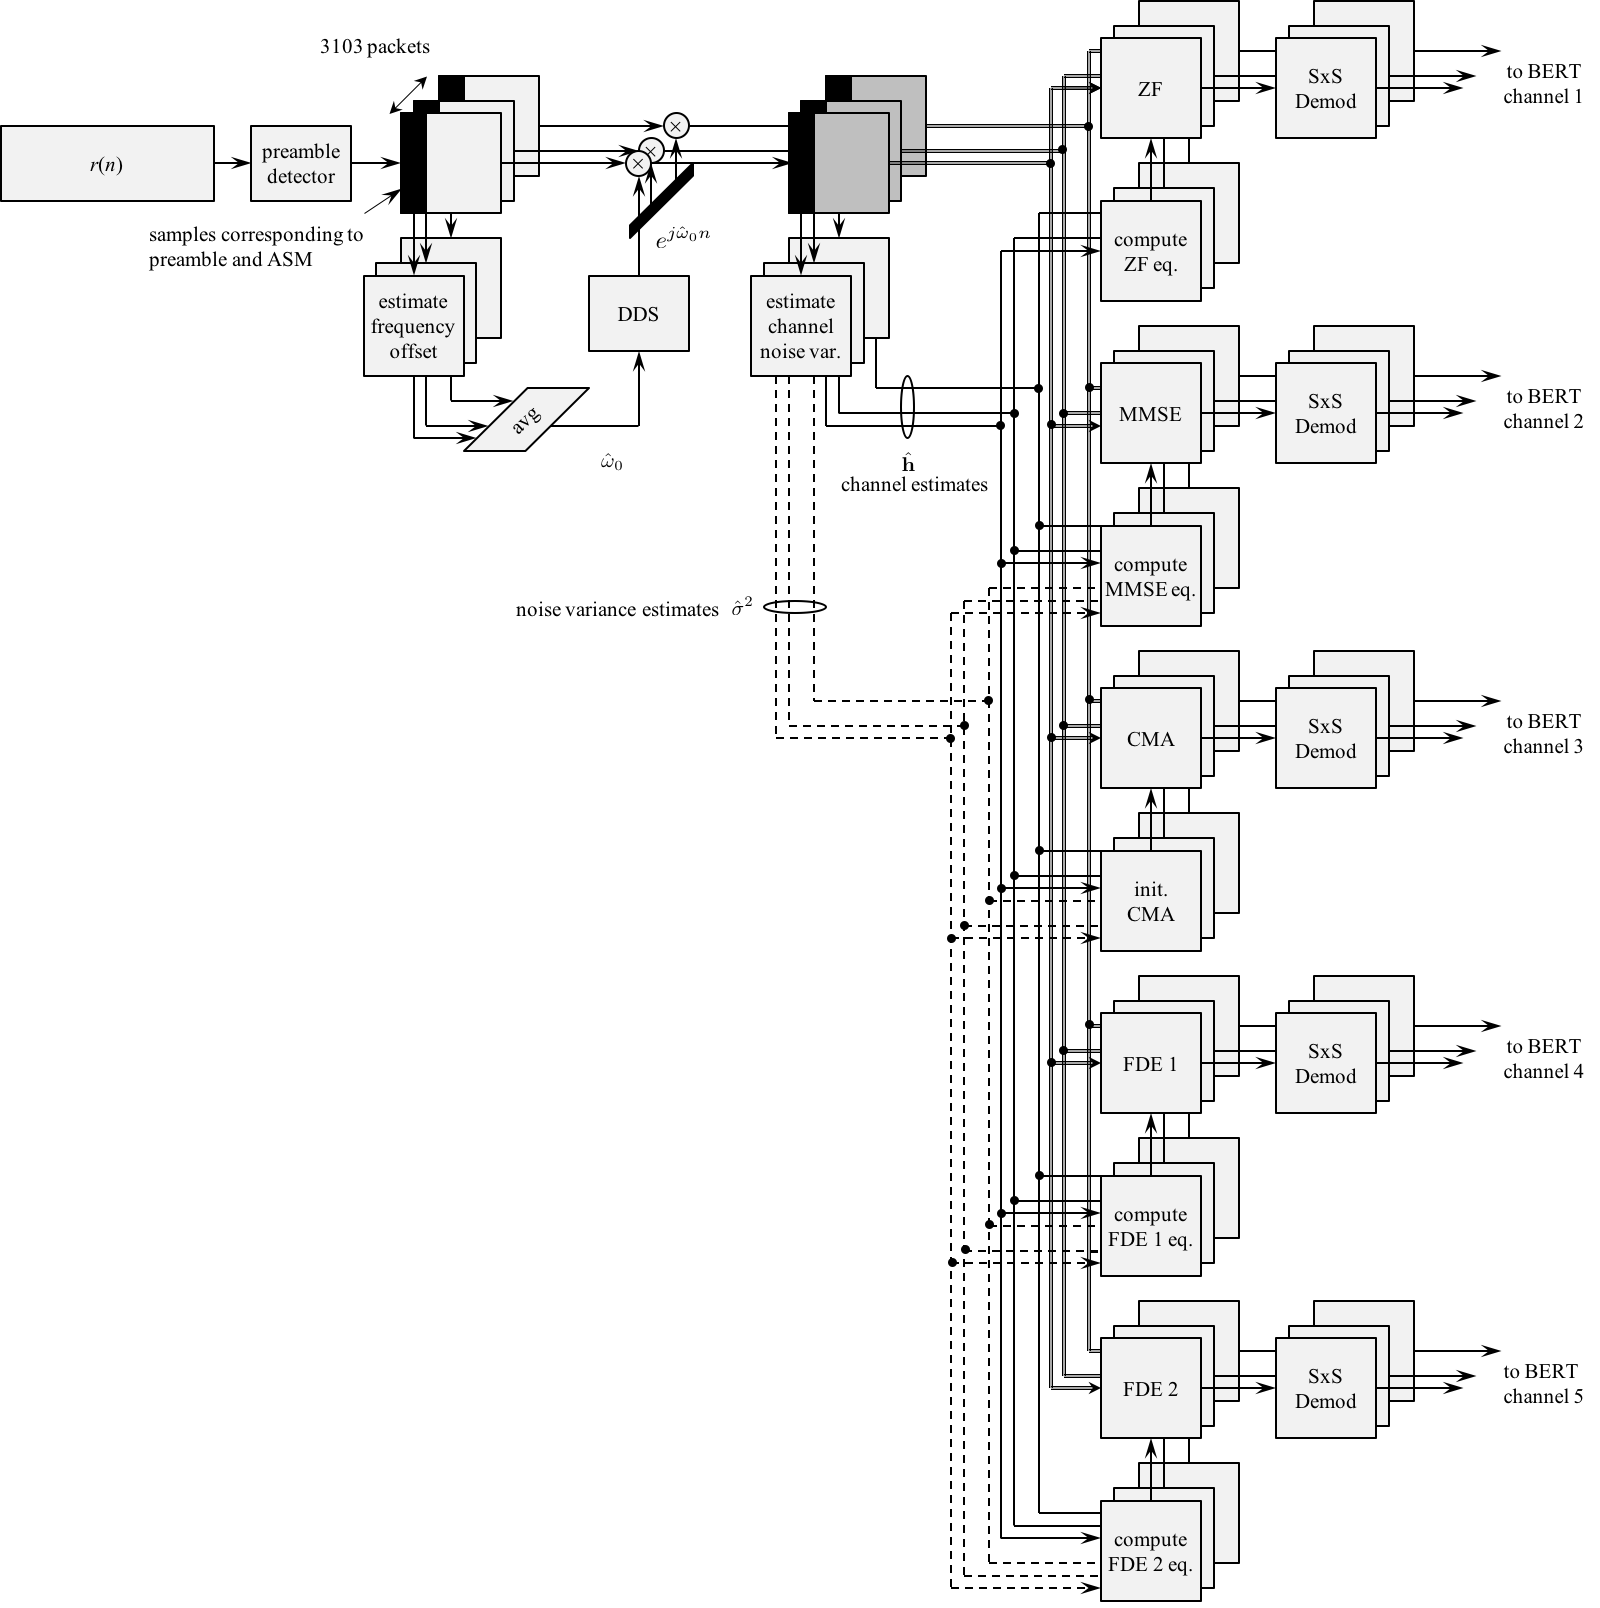
\includegraphics[width=\textwidth]{figures/gpu/signal-flow-gpu-2}
%	\caption{A block diagram illustrating organization of the algorithms in the GPU.}
%	\label{fig:signal-flow-gpu}
%\end{figure}

%\section{GPU Algorithm Implementation}
%Once the $39{,}321{,}600$ complex floating point received samples are transferred from the FPGA to the host CPU, they are transferred to the Tesla k40 GPU shown in Figure \ref{fig:paq-hardware-overview} in Chapter \ref{sec:hardware}.
%With the samples tresferred to the k40 GPU, all the algorithms are ready to run.
%Figure \ref{fig:software-algorithmBlockDiagramSimple} shows the steps in the PAQ GPU implementation. 
%\begin{figure}
%	\centering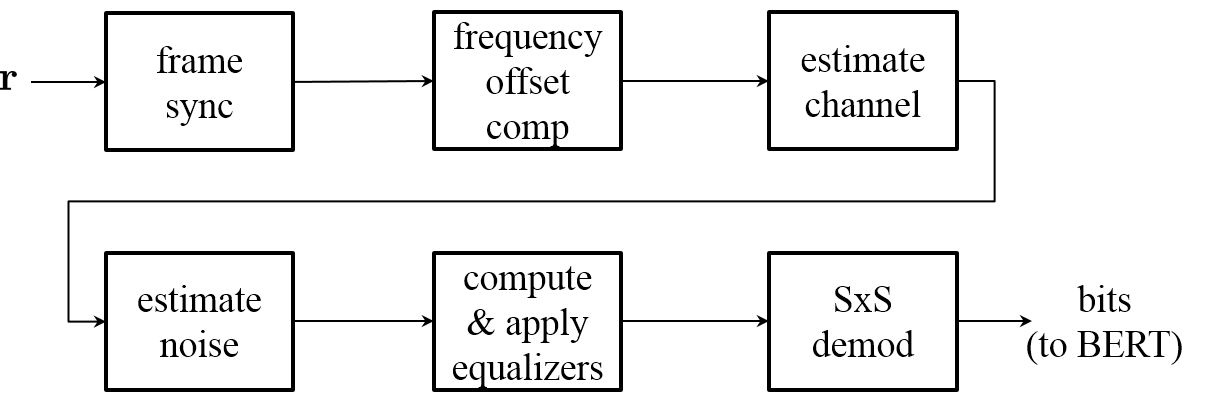
\includegraphics[width=\textwidth/10*8]{figures/gpu/software-algorithmBlockDiagramSimple.png}
%	\caption{A block diagram illustrating algorithm flow}
%	\label{fig:software-algorithmBlockDiagramSimple}
%\end{figure}
%
%The frame sync block in Figure \ref{fig:software-algorithmBlockDiagramSimple} uses a preamble detector to find the indices for the start of the $3,103$ packets in the received. 
%The frame sync block also packetizes the data into $L_{pkt}$ portions of $12,672$ samples.
%Before the the channel can be estimated, the frequency offset is removed because so the channel estimator is accurate.
%The channel and noise are then estimated using the preamble.
%With the preambles located, the frequency offset and the channel response and noise variance estimated, the 5 studied equalizers are calculated using the estimated channel and noise variance.
%
%\subsection{Convolution GPU Implementation}
%A common tool in digital signal processing is the discrete time convolution sum.
%A convolution sum applies a finite impulse response (FIR) filter to a signal.
%The FIR filter might be low pass, high pass or an equalizer.
%Applying a FIR filter $\mathbf{h}$ to a signal vector $\mathbf{x}$ is
%\begin{equation}
%y(n) = \left(\mathbf{x}*\mathbf{h}\right)(n) = \sum_{m=0}^{L_h-1} x(n) h(n-m)
%\label{eq:time-convolution}
%\end{equation}
%when $\mathbf{h}$ is $L_h$ long with the center tap $n_0$. 
%Figure \ref{fig:conv-n_0} shows the convolution of $\mathbf{x}$ with $\mathbf{h}$ results in $\mathbf{y}$.
%The desired portion of $\mathbf{y}$ is $L_y$ long and pruned out starting at $n_0$ (the center tap index of $\mathbf{h}$).
%The grey boxes in Figure \ref{fig:conv-n_0} are the pruned samples of $\mathbf{y}$.
%
%Convolution can also be expressed as the matrix operation
%\begin{equation}
%\begin{bmatrix}
%y(0) \\
%y(1) \\
%\vdots \\
%y(L_x-2) \\
%y(L_x-1)
%\end{bmatrix} = 
%\begin{bmatrix}
%x(n_0) & x(n_0-1) & \cdots & x(n_0-(L_h-1))\\
%x(n_0+1) &x(n_0) & \cdots & x(n_0-L_h) \\
%\vdots & \vdots &\ddots &\vdots\\
%\\
%  & & & x(n_0) \\
%  & & & x(n_0+1) \\
% \vdots & \vdots & & \vdots \\
% x(L_x+n_0) & x(L_x+n_0+1) & \cdots & x(L_x+L_h+n_0-1)
%\end{bmatrix}
%\begin{bmatrix}
%h(0)\\
%h(1)\\
%\vdots\\
%h(L_h-1)
%\end{bmatrix}
%\label{eq:conv-matrix}
%\end{equation} 
%or
%\begin{equation}
%\mathbf{y} = \mathbf{X}\mathbf{h}.
%\label{eq:matrix_conv}
%\end{equation}
%where the result $\mathbf{y}$ is the matrix multiplication of the $L_x \times L_h$ convolution matrix $\mathbf{X}$ and filter coefficients $\mathbf{h}$.
%\begin{figure}
%	\centering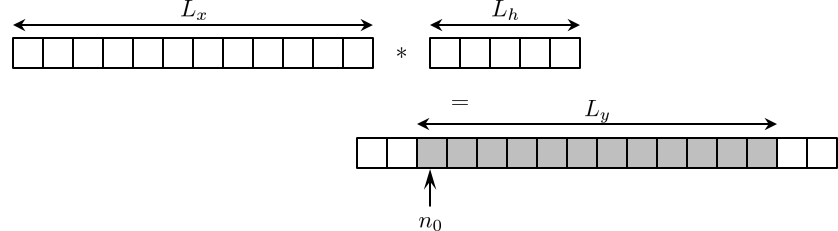
\includegraphics[width=\textwidth/10*8]{figures/gpu/conv-n_0.png}
%	\caption{The convolution of the vector $\mathbf{x}$ with the vector $\mathbf{h}$ results 					in the vector $\mathbf{y}$. The grey desired portion of $\mathbf{y}$ is from 					$n_0$ to $n_0+L_y$.}
%	\label{fig:conv-n_0}
%\end{figure}
%
%With a large data set or filter, implementing convolution with Fast Fourier Transforms (FFTs) is computationally more efficient than using equation \eqref{eq:time-convolution} or \eqref{eq:matrix_conv}.
%FFTs are used to compute a $N$ point Discrete Fourier Transform (DFT) quickly and efficiently.
%\begin{equation}
%\mathbf{x}*\mathbf{h} = \text{IFFT}_N\Big[\text{FFT}_N\left[\mathbf{x}\right]\cdot\text{FFT}_N\left[\mathbf{h}\right]\Big]
%\label{eq:fft-conv}
%\end{equation}
%The FFT algorithm is most efficient when $N$ is a power of $2$: $2$, $4$, $8$, $16$, $32$, ect.
%The FFT length $N$ must be greater or equal to $L_x + L_h - 1$.
%Each vector, $\mathbf{x}$ and $\mathbf{h}$ must be zero padded to the length $N$.
%
%The block diagram in Figure \ref{fig:conv_FFT_block} shows how a convolution is implemented in a GPU using FFTs.
%To implement the zero pad block, the GPU launches $L_x$ or $L_h$ threads to fill a zero initialized vector.
%The FFT block is done with a cuFFT library to compute the forward FFT \cite{nvidia-CUDAdoc:2015}.
%The FFTs of $\mathbf{x}$ and $\mathbf{h}$ are multiplied using a hadamard point to point multiply by launching $N$ GPU threads.
%With the FFTs multiplied, the GPU calls an inverse FFT or IFFT from the cuFFT library.
%The GPU then launches $L_y$ threads to prune out the desired portion of the IFFT.
%\begin{figure}
%%	\centering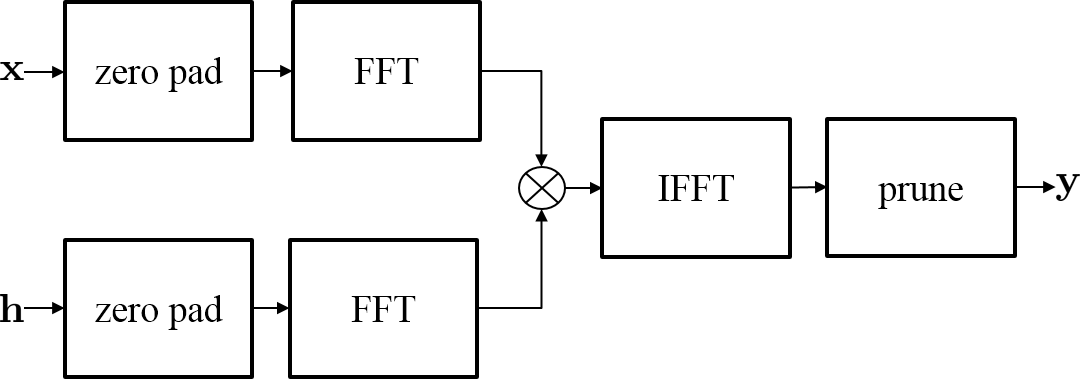
\includegraphics[width=\textwidth/10*8]{figures/gpu/conv_FFT_block.png}
%	\caption{Block diagram showing how the convolution of two vectors can be done using FFTs.}
%	\label{fig:conv_FFT_block}
%\end{figure}
%\begin{figure}
%	\centering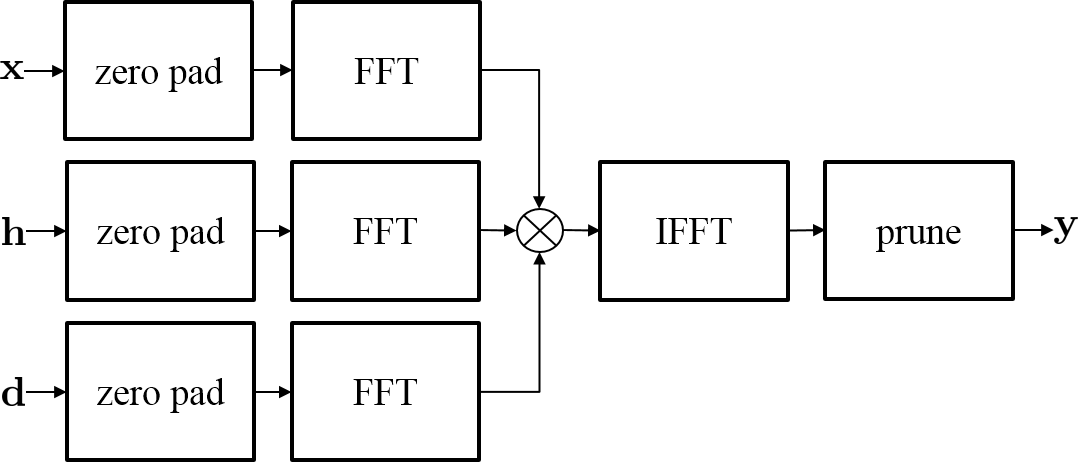
\includegraphics[width=\textwidth/10*8]{figures/gpu/conv_FFT_block3.png}
%	\caption{Block diagram showing how the convolution of three vectors can be done using FFTs.}
%	\label{fig:conv_FFT_block3}
%\end{figure}
%
%To convolove more than two vectors, another row of zero pad and FFT blocks must be added for each additional vector and $n_0$ is adjusted accordingly.
%Figure \ref{fig:conv_FFT_block3} shows the block diagram from convolving three vectors $\mathbf{x}$, $\mathbf{h}$ and $\mathbf{d}$.
%For simplicity and clarity only, the blocks in Figure \ref{fig:conv_simple_block} will be shown from now on instead of Figures \ref{fig:conv_FFT_block} or \ref{fig:conv_FFT_block3}.
%\begin{figure}
%	\centering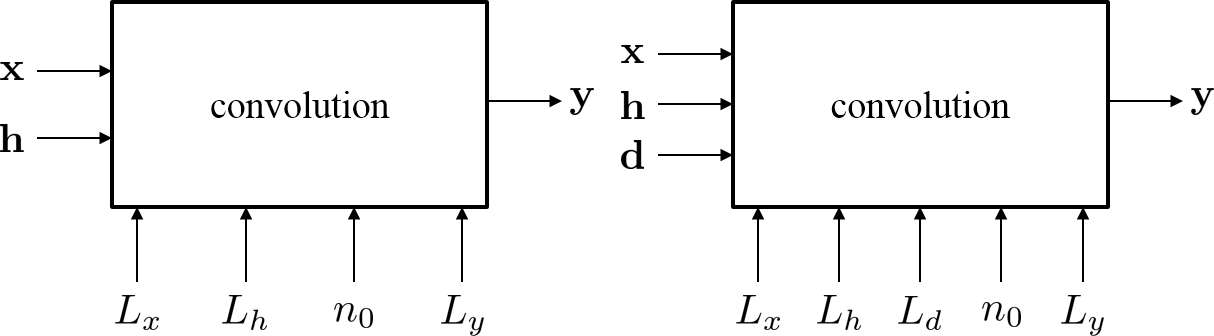
\includegraphics[width=\textwidth/10*9]{figures/gpu/conv_simple_block.png}
%	\caption{Instead of showing Figure \ref{fig:conv_FFT_block} or \ref{fig:conv_FFT_block3}, the single block convolution is shown.}
%	\label{fig:conv_simple_block}
%\end{figure}
%
%\subsection{Estimator GPU Implementation}
%Before calculating equalizers to combat multipath the GPU must find each packet and synchronize the received samples to used the preamble and ASM.
%The equalizers are calculated based on the channel and noise estimates.
%The channel and noise estimators are sensitive to frequency offset.
%The frequency offset must be removed if it is present in the received samples to have accurate estimates.

\subsubsection{Frame Synchronization}
To compute preamble assisted equalizers, estimators use the preamble to estimate various parameters. 
The iNET packet is comprised of three different sections: preamble, asynchronous marker (ASM) and the data. 
The packet and received sample structure is shown in Figure\ref{fig:packet}.
\begin{figure}
	\centering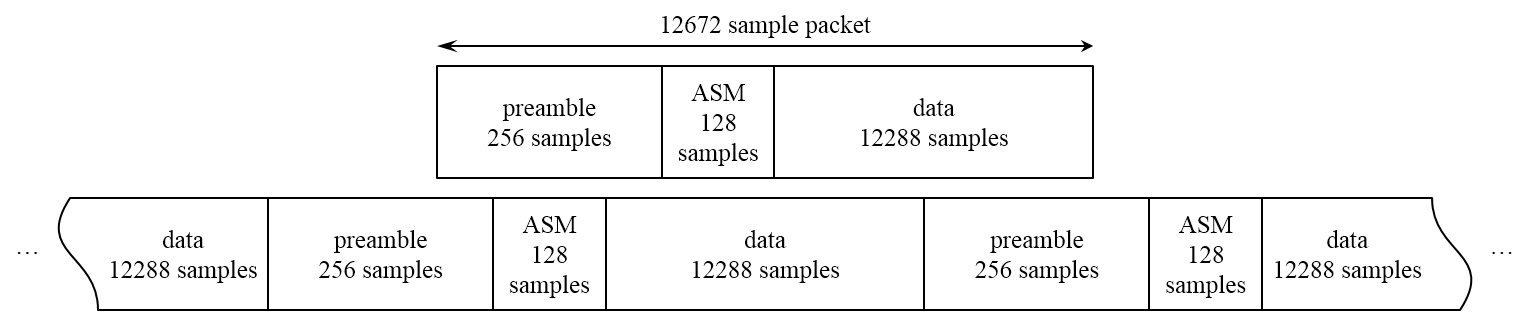
\includegraphics[width=\textwidth]{figures/gpu/packet.png}
	\caption{The iNET packet structure.}
	\label{fig:packet}
\end{figure}

The goal of the frame synchronization step is to synchronize the received samples into frames or packets by locating the preambles. 
To give an overview of the frame synchronization step, synchronization of the received samples is explained using a preamble detector and search algorithms to packetize the received samples. 
To find the preambles in the batch, a preamble detector is used to compute the sample correlation function between the received samples and the preamble. 
Search algorithms then search the correlation function for sample indices that correlate strongest to the preamble. These indices are the starting indices of each packet in the received samples. 
Finally, using the starting indices of each packet, received samples are structured and synchronized into frames or packets.

The first step in the frame synchronizer is to compute the sample correlation between the received samples and the preamble.
A lower complexity preamble detector is shown in equation \eqref{eq:L-4}-\eqref{eq:L-pedone-geoghegan-4} in section \ref{sec:estimators} and repeated here for convenience.
\begin{equation}
	L(n) = \sum_{m=0}^{7}
		\left[ I^2(n,m) + Q^2(n,m) \right]
	\label{eq:gpu-L-4}
\end{equation}
where
\begin{multline}
	I(n,m) \approx \sum_{\ell\in\mathcal{L}_1}r_R(\ell+32m+n)
			- \sum_{\ell\in\mathcal{L}_2}r_R(\ell+32m+n)
			+ \sum_{\ell\in\mathcal{L}_3}r_I(\ell+32m+n)
			- \sum_{\ell\in\mathcal{L}_4}r_I(\ell+32m+n)
			\\
			+ 0.7071 \left[
				\sum_{\ell\in\mathcal{L}_5}r_R(\ell+32m+n)
				- \sum_{\ell\in\mathcal{L}_6}r_R(\ell+32m+n)
			\right. \\
			\left.
				+ \sum_{\ell\in\mathcal{L}_7}r_I(\ell+32m+n)
				- \sum_{\ell\in\mathcal{L}_8}r_I(\ell+32m+n)
			\right],
	\label{eq:gpu-L-pedone-geoghegan-2}
\end{multline}
\begin{multline}
	Q(n,m) \approx \sum_{\ell\in\mathcal{L}_1}r_I(\ell+32m+n)
			- \sum_{\ell\in\mathcal{L}_2}r_I(\ell+32m+n)
			\\
			- \sum_{\ell\in\mathcal{L}_3}r_R(\ell+32m+n)
			+ \sum_{\ell\in\mathcal{L}_4}r_R(\ell+32m+n)
			\\
			+ 0.7071 \left[
				\sum_{\ell\in\mathcal{L}_5}r_I(\ell+32m+n)
				- \sum_{\ell\in\mathcal{L}_6}r_I(\ell+32m+n)
			\right. \\
			\left.
				- \sum_{\ell\in\mathcal{L}_7}r_R(\ell+32m+n)
				+ \sum_{\ell\in\mathcal{L}_8}r_R(\ell+32m+n)
			\right]
		\label{eq:gpu-L-pedone-geoghegan-3}
\end{multline}
with
\begin{equation}
	\begin{split}
	\mathcal{L}_1 &= \{ 0, 8, 16, 24 \}\\
	\mathcal{L}_2 &= \{ 4, 20 \}\\
	\mathcal{L}_3 &= \{ 2, 10, 14, 22 \}\\
	\mathcal{L}_4 &= \{ 6, 18, 26, 30 \}\\
	\mathcal{L}_5 &= \{ 1, 7,  9, 15, 17, 23, 25, 31 \}\\
	\mathcal{L}_6 &= \{ 3, 5, 11, 12, 13, 19, 21, 27, 28, 29 \}\\
	\mathcal{L}_7 &= \{ 1, 3,  9, 11, 12, 13, 15, 21, 23 \}\\
	\mathcal{L}_8 &= \{ 5, 7, 17, 19, 25, 27, 28, 29, 31 \}.
\end{split}
\label{eq:gpu-L-pedone-geoghegan-4}
\end{equation}

The preamble detector is implemented in the GPU in two kernels as shown by the dotted box in Figure \ref{fig:preambleBlock}.
The first kernel computes the inner summations and the second computes the outer summation.
\begin{figure}
	\centering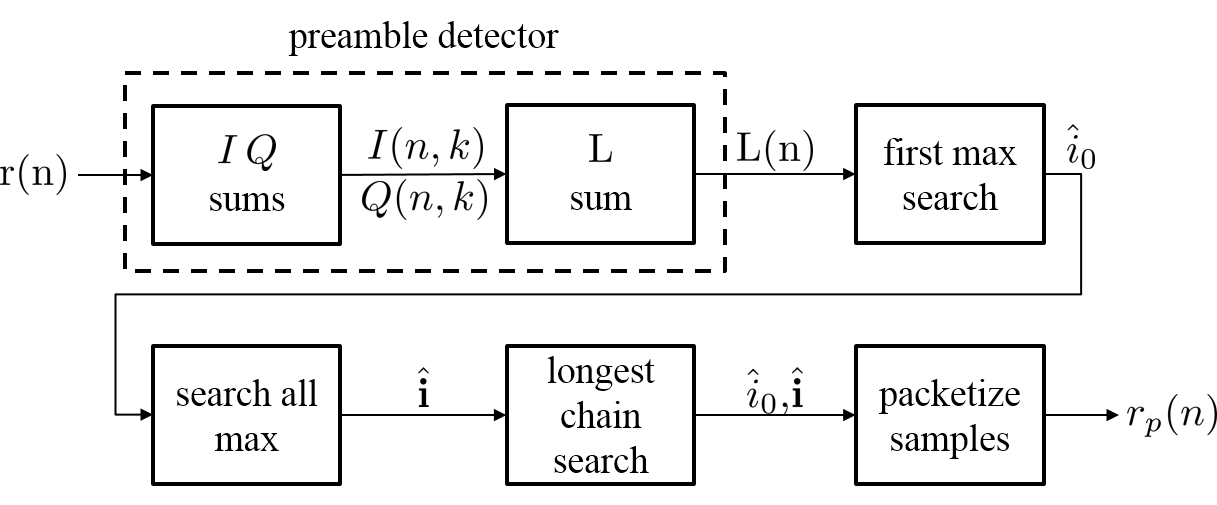
\includegraphics[width=\textwidth/10*8]{figures/gpu/preambleBlock.png}
	\caption{The block diagram for the frame synchronization implementation.}
	\label{fig:preambleBlock}
\end{figure}

The inner summation, as defined in equations \eqref{eq:gpu-L-pedone-geoghegan-2}-\eqref{eq:gpu-L-pedone-geoghegan-4}, computes an $I$ and $Q$ pair.
A single $I$ and $Q$ pair is computed by summing 32 scaled real or imaginary parts of received samples.
For each received sample an $I$ and $Q$ pair is computed.

The outer summation, as defined in equation \eqref{eq:gpu-L-4}, computes the reduced complexity maximum likelihood correlation $L$.
One sample of $L$ is computed by summing 8 squared then summed $I$ and $Q$ pairs.
For each received sample $L$ is computed.

Figure \ref{fig:L_2_packets} shows an example of the first $2\times L_{pkt} $ samples of $L$.
The local maximums in $L$ in the figure indicate a preamble starts at the maximum's sample index.
The first local maximum is at sample index $7040$, indicating the first packet starts at that index.
The figure also shows the second packet starts at sample index $19712$.
The difference between these sample indices is $ L_{pkt} $, this difference agrees with the packet length shown in Figure \ref{fig:packet}.
\begin{figure}
	\centering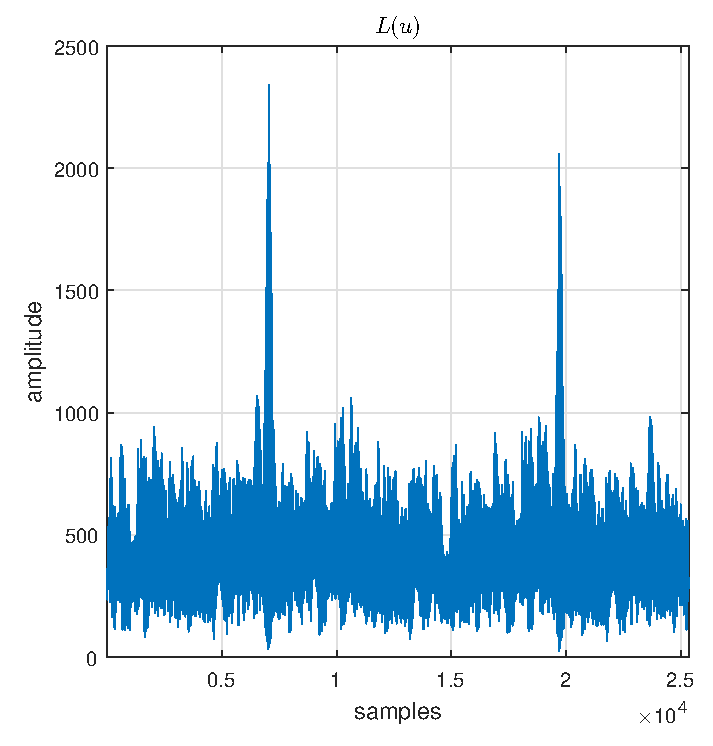
\includegraphics[width=5in]{figures/gpu/L_2_packets.eps}
	\caption{The output of the Preamble Detector $L(u)$.}
	\label{fig:L_2_packets}
\end{figure}

Because of the structure of the preamble, the preamble detector output $L$ has some unique properties.
The Figures in \ref{fig:L_corr_creepy} show the correlation function around an expected preamble location.
The correlation functions have peaks every 32 samples because the preamble bit sequence comprises eight repetitions of the 16-bit pattern $\text{CD98}_\text{hex}$.
The repetitive structure causes one main correlation peak with seven side peaks.

When ideal samples are received the preamble detector output looks like Figure \ref{fig:L_corr_creepy}(a).
The structure of the correlation peaks still occur when the signal to noise ratio is low, as shown in Figure \ref{fig:L_corr_creepy}(b).
But when the signal to noise ratio is low and major multipath distortion happen, the correlation peaks look like Figures \ref{fig:L_corr_creepy}(c) and (d).
The structure of the correlation peaks can cause a simple algorithm to find an incorrect preamble starting location.

In the worst case scenario, a simple algorithm might find an incorrect preamble index by searching a poorly placed search window.
A poorly placed window might search the large side correlation peaks from Figure \ref{fig:L_corr_creepy}(a) and the small main correlation peaks from Figures \ref{fig:L_corr_creepy}(c) or (d).
Because the first three side peaks in Figure \ref{fig:L_corr_creepy}(a) are much taller than the main peak in Figures \ref{fig:L_corr_creepy}(c) and (d), an incorrect preamble starting indices will result if search windows are not defined safely.
\begin{figure}
	\begin{center}
		\begin{tabular}{cc}
			\begin{minipage}[c]{3in}
				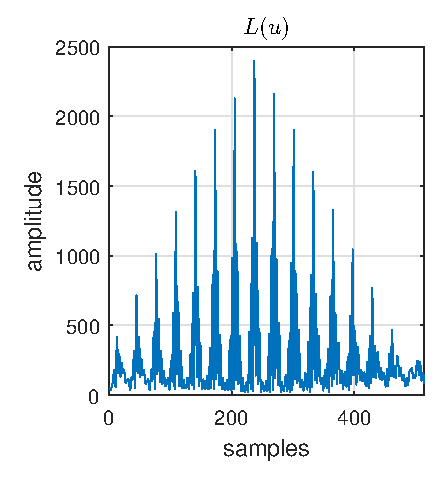
\includegraphics[width=3in]{figures/gpu/L_corr_8_clean.eps}
			\end{minipage} 
			&  
			\begin{minipage}[c]{3in}
				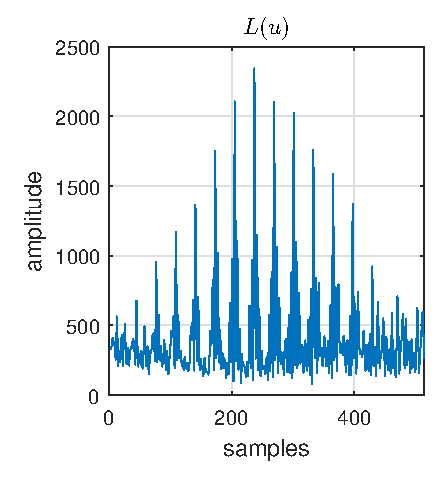
\includegraphics[width=3in]{figures/gpu/L_corr_8_noise.eps}
			\end{minipage} \\[12pt]
			
			\quad\quad\quad\quad(a)
			&
			\quad\quad\quad\quad(b) \\[12pt]
			
			\begin{minipage}[c]{3in}
				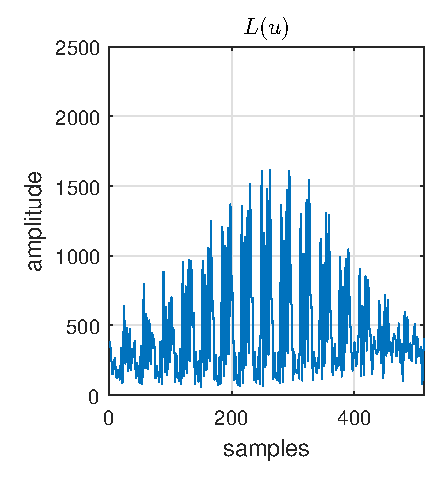
\includegraphics[width=3in]{figures/gpu/L_corr_17_creepy.eps}
			\end{minipage} 
			&  
			\begin{minipage}[c]{3in}
				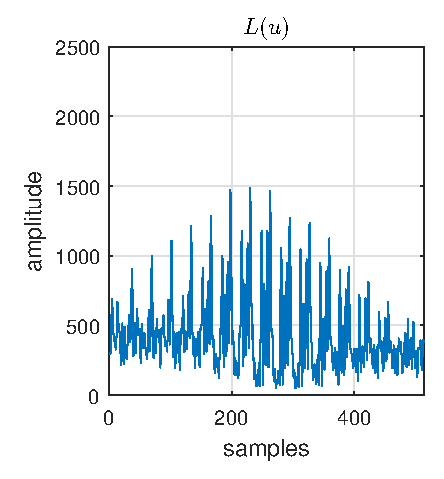
\includegraphics[width=3in]{figures/gpu/L_corr_18_creepy.eps}
			\end{minipage} \\[12pt]
			
			\quad\quad\quad\quad(c)
			&
			\quad\quad\quad\quad(d)
			
		\end{tabular}
	\end{center}
	\caption{Detailed view of $L(u)$. 
			(a): correlation peaks of a distortion free and noiseless signal; 
			(b): correlation peaks of a distortion free but noisy signal with $E_b/N_0 = 0$dB; 
			(c): correlation peaks of a distorted and noisy signal with $E_b/N_0 = 0$dB;
			(d): correlation peaks of a distorted and noisy signal with $E_b/N_0 = 0$dB}
	\label{fig:L_corr_creepy}
\end{figure}

To prevent searching multiple preamble correlation peaks, search windows should only search the correlation peak of one preamble.
To ensure the correlation peaks from only one preamble is searched, windows of length $ L_{pkt} $ are centered on expected preamble starting locations.
Figure \ref{fig:L_windows} shows an example of safe search windows centered on expected preamble starting locations.
\begin{figure}
	\centering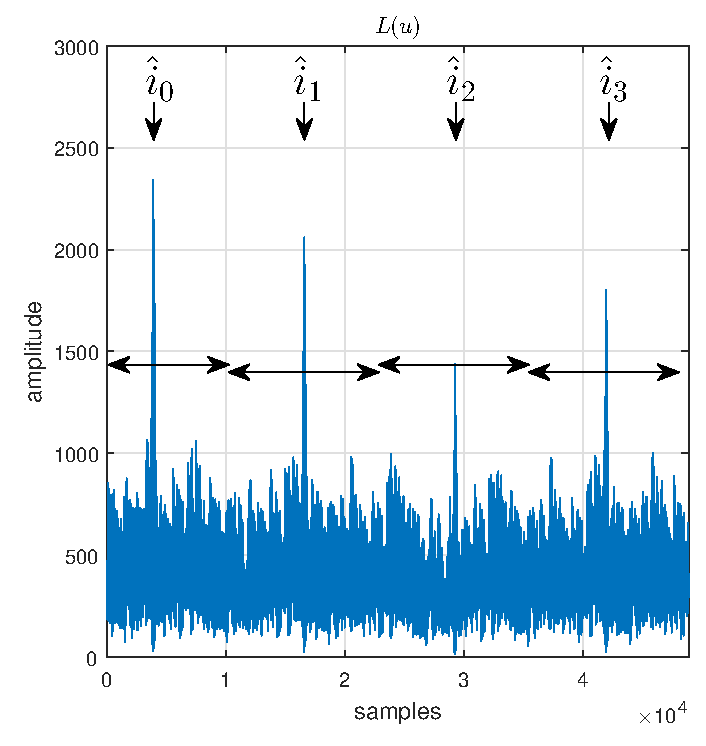
\includegraphics[width=5in]{figures/gpu/L_windows.eps}
	\caption{Safe search windows defined to search only one preamble correlation peak.}
	\label{fig:L_windows}
\end{figure}

To define safe search windows, a rough estimate of the preamble starting locations is made.
The GPU launches a kernel with one thread to search for the maximum in the first $ L_{pkt} $ samples of the received samples.
The maximum index is saved as $\hat{i}_0$.
$\hat{i}_0$ is used to make a rough estimate for all the preamble staring locations by building a vector defined as
\begin{align}
\hat{\mathbf{i}}
=     
\begin{bmatrix}
\hat{i}_0 + 0\times L_{pkt}  			\\
\hat{i}_0 + 1\times L_{pkt}  		\\
\vdots			\\
\hat{i}_0 + 3102\times L_{pkt}  		\\
\hat{i}_0 + 3103\times L_{pkt}  		
\end{bmatrix}
\label{eq:preamble_det_i_hat}
\end{align}

With rough estimates of where the preambles should be located, the GPU searches safe windows of $L$ for local maximums.
On local maximum is found in each search window by centering each window on elements from $\hat{\mathbf{i}}$.
The GPU launches one thread per search window to find the local maximum and save its sample index in $\hat{\mathbf{i}}$.
The vector $\hat{\mathbf{i}}$ has the sample indices for $3103$ local maximums that should be $ L_{pkt} $ samples apart.

Because of noise and multipath, the sample indices in $\hat{\mathbf{i}}$ are not the ideal $ L_{pkt} $ samples.
The GPU launches one thread to search $\hat{\mathbf{i}}$ for the longest chain of perfectly spaced indices.
The modulo of the last index in the longest chain of indices spaced $ L_{pkt} $ samples apart is the best estimate for $\hat{i}_0$.
Once again, $\hat{i}_0$ is updated with the best estimated first preamble starting location.
The vector $\hat{\mathbf{i}}$ is also updated again as in equation \eqref{eq:preamble_det_i_hat}. 

Now with the best estimate of the preamble starting locations, the received samples can be packetized and synchronized.
Figure \ref{fig:packets_in_batch} shows the relationship of $\hat{\mathbf{i}}$ and $\boldsymbol{r}$.
Using $\hat{\mathbf{i}}$, the GPU launches one thread per received sample to packetize $\boldsymbol{r}$ into $\boldsymbol{r}_p$ as shown in Figure \ref{fig:packetized}. The structure of $r_p$ majorly simplifies indexing and removes the need for $\hat{\mathbf{i}}$.
\begin{equation}
\boldsymbol{r}_p = 
\begin{bmatrix}
r(\hat{i}_0) 			\\
r(\hat{i}_0+1) 		\\
\vdots			\\
r(\hat{i}_0+12670)\\
r(\hat{i}_0+12671)\\
r(\hat{i}_1) 			\\
r(\hat{i}_1+1) 		\\
\vdots			\\
r(\hat{i}_{3103}+12670)\\
r(\hat{i}_{3103}+12671)\\
\end{bmatrix}
\end{equation}

\begin{figure}
	\centering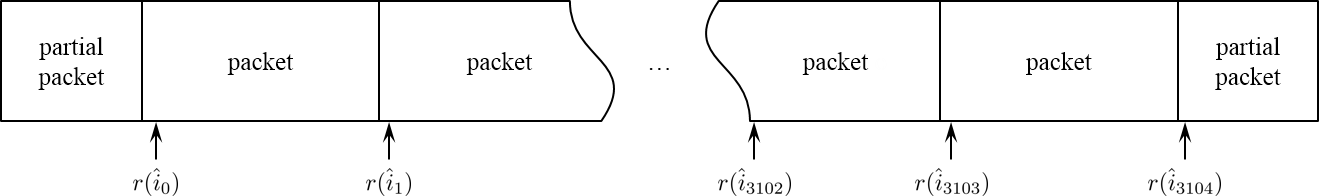
\includegraphics[width=\textwidth/10*8]{figures/gpu/packets_in_batch.png}
	\caption{The starting sample index for each packet in the batch.}
	\label{fig:packets_in_batch}
\end{figure}
\begin{figure}
	\centering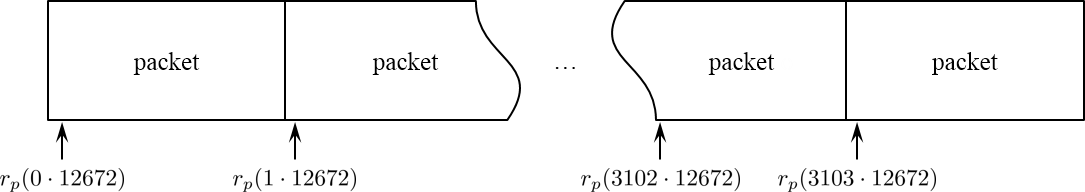
\includegraphics[width=\textwidth/10*8]{figures/gpu/packetized.png}
	\caption{The packetized structure of the received signals after the frame synchronization step.}
	\label{fig:packetized}
\end{figure}

The steps in Figure \ref{fig:preambleBlock} synchronize the received samples $r$ into $r_p$ by using a preamble detector.
The output of the preamble detector, $L$, is searched for local maximums.
Imperfect spacing of local maximums is fixed by finding the longest chain of perfectly spaced indices in $\hat{\mathbf{i}}$.
The received samples are then packetized based on the corrected preamble spacing.

\clearpage

\subsubsection{Frequency Offset Compensation}
\label{sec:jeffs_frequencyoffsetestimator}
As discussed in section \ref{sec:joint-ML-estimator}, all the estimators depend on atleast one of the other parameters.
Estimating the frequency offset using the periodic properties of the preamble gives an accurate estimate, even in multipath.
The frequency offset is estimated using the data-aided frequency offset estimator in equation \eqref{eq:ML-w-final3}.
To compensate for the frequency offset, the received samples are rotated by the negative of estimated frequency offset.
The data-aided frequency offset estimator equation is repeated here for convenience.
\begin{equation}
	\hat{\omega}_0 = \frac{1}{L_q} \arg\left\{ \sum_{n=i+2L_q}^{i+7L_q-1} r(n)r^\ast(n-L_q)\right\}
	\label{eq:jeff-ML-w-final3}
\end{equation}
where
$\hat{\omega}_0$ is the frequency offset estimate for a single packet.
The summation in equation \eqref{eq:jeff-ML-w-final3} can be reformulated in terms of an inner product
\begin{equation}
	\hat{\omega}_0 = \frac{1}{L_q} \arg\left\{ \mathbf{r}_{p1}^T \mathbf{r}^\ast_{p2}  \right\}.
	\label{eq:jeff-ML-w-final3_reformed}
\end{equation}
where 
\begin{align}
\mathbf{r}_{p1}
=     
\begin{bmatrix}
r_p(2L_q) 			\\
r_p(2L_q+1) 		\\
\vdots			\\
r_p(7L_q - 2)\\
r_p(7L_q - 1)
\end{bmatrix}
\label{eq:freq_offset_r1}
\end{align}
\begin{align}
\mathbf{r}^\ast_{p2}
=     
\begin{bmatrix}
r^\ast_p(L_q) 			\\
r^\ast_p(L_q+1) 		\\
\vdots			\\
r^\ast_p(6L_q - 2)\\
r^\ast_p(6L_q - 1)
\end{bmatrix}
\end{align}

Reformulating the estimator into an inner product isn't only simpler, it is also much faster in the GPU.
The GPU uses an extremely fast and efficient CUDA Basic Linear Algebra Subprogram (CUBLAS) library to compute the inner product \cite{nvidia-CUDAdoc:2015}.
Figure \ref{fig:frequencyOffsetBlock} shows how equation \eqref{eq:jeff-ML-w-final3_reformed} is implemented in GPU kernels.
The GPU strips $\mathbf{r}_{p1}$ and $\mathbf{r}^\ast_{p2}$ from the received packetized samples by launching one thread per packetized sample.
\begin{figure}
	\centering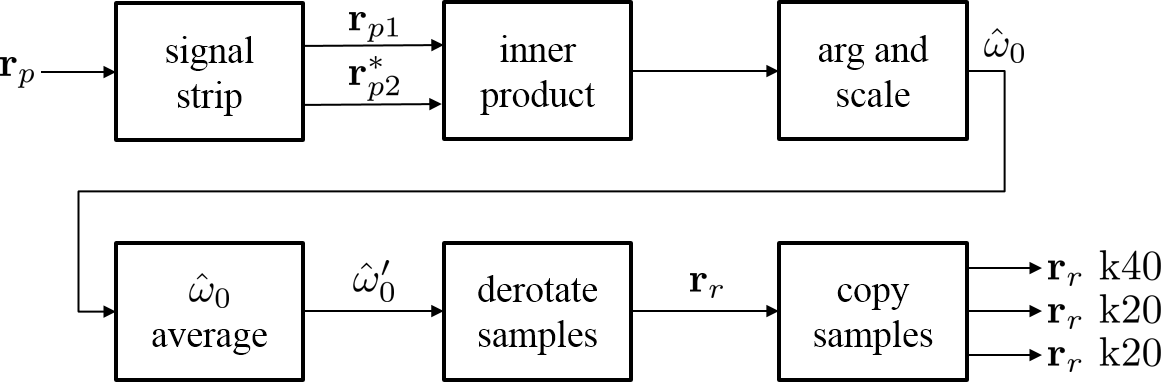
\includegraphics[width=\textwidth/10*8]{figures/gpu/frequencyOffsetBlock.png}
	\caption{The block diagram for the Frequency Offset estimator and sample rotation implementation.}
	\label{fig:frequencyOffsetBlock}
\end{figure}

The GPU computes the inner product of $\mathbf{r}_{p1}$ and $\mathbf{r}^\ast_{p2}$ using a batched CUBLAS operation.
The arg and scale GPU kernel launches one thread per packet to compute the scaled angle of the inner product for each packet.
The scaled angle of each packet is saved in the vector $\hat{\boldsymbol{\omega}}_0$.

In aeronautical telemetry, the frequency offset can be assumed to be constant over two seconds.
Because of this assumption, one frequency offset estimate is obtained by averaging all the offsets in a batch.
The GPU launches one thread to compute the average of the vector $\hat{\boldsymbol{\omega}}_0$ and save the average in the scalar value $\hat{\omega}^\prime_0$.

The averaged frequency offset $\hat{\omega}^\prime_0$ is used to compensate for the frequency offset.
The frequency offset compensation can be done with the matrix $\boldsymbol{\Omega}_r$ the rotations due to the frequency offset are in matrix notation using 
\begin{equation}
	\boldsymbol{r}_r = \boldsymbol{\Omega}_r \boldsymbol{r}_p = 
	\begin{bmatrix} e^{-j\hat{\omega}^\prime_0(0)} & & \\ & \ddots & \\ & & e^{-j\hat{\omega}^\prime_0(3103\times L_{pkt} -1)} \end{bmatrix}
\begin{bmatrix}
r_p(0) 			\\
\vdots			\\
r_p(3103\times L_{pkt} -1)
\end{bmatrix}.
	\label{eq:jeff-Omega_0-matrix1}
\end{equation}

Implementing equation \eqref{eq:jeff-Omega_0-matrix1} in GPUs would use an extreme amount of memory and computation because of the size and dimension of $\boldsymbol{\Omega}_r$.
Instead, the GPU launches one thread per packetized sample to rotate the packetized sample by $-\hat{\omega}^\prime_0$.
\begin{equation}
r_r(n) = r_p(n) \times e^{-j \hat{\omega}^\prime_0 n}
\end{equation}

With the frequency offset compensation done, the samples are transferred over the PCIe bus from the Tesla k40 GPU to the two Tesla k20 GPUs, shown as the last block in Figure \ref{fig:frequencyOffsetBlock}.


\subsubsection{Channel Estimation}
\begin{figure}
	\centering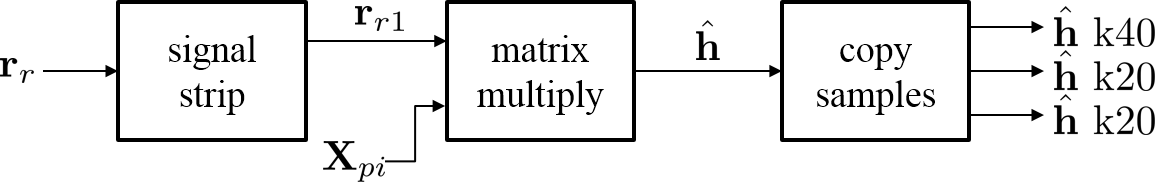
\includegraphics[width=\textwidth/10*8]{figures/gpu/channelBlock.png}
	\caption{The block diagram for the Channel estimator.}
	\label{fig:channelBlock}
\end{figure}
As mentioned in \ref{sec:joint-ML-estimator}, the channel cannot be estimated with a frequency offset in the received samples.
With the offset removed, the channel can accurately be estimated.
Equation \eqref{eq:ML-h-final2} is used to compute the channel estimate.
The equation is repeated below for convenience.
\begin{equation}
	\hat{\mathbf{h}} = \left( \mathbf{X}^\dag\mathbf{X} \right)^{-1} \mathbf{X}^\dag\hat{\boldsymbol{\Omega}}_0^\dag \mathbf{r}
\label{eq:jeff-ML-h-final2}
\end{equation}

The channel estimator was originally formulated assuming the received samples still had a frequency offset.
The samples in the GPU have already compensated for the offset and \eqref{eq:jeff-ML-h-final2} is reformed into
\begin{equation}
	\hat{\mathbf{h}} = \left( \mathbf{X}^\dag\mathbf{X} \right)^{-1} \mathbf{X}^\dag \mathbf{r}_{r1}.
\label{eq:channel_reformed_no_freq}
\end{equation}
where
\begin{align}
\mathbf{r}_{r1}
=     
\begin{bmatrix}
r_r(N_2) 		\\
r_r(N_2+1) 		\\
\vdots			\\
r_r(L_p - N_1 - 2)\\
r_r(L_p - N_1 - 1)
\end{bmatrix}
\end{align}

The matrix $\mathbf{X}$ is the $(L_p+L_a-N_1-N_2)\times (N_1+N_2+1)$ convolution matrix
formed from the iNet preamble and ASM samples. 
The psnudo inverse of $\mathbf{X}$, $\left( \mathbf{X}^\dag\mathbf{X} \right)^{-1} \mathbf{X}^\dag$ is computed once and saved as $\mathbf{X}_{pi}$.
Equipped with $\mathbf{X}_{pi}$ the channel estimator can be reformed again into
\begin{equation}
	\hat{\mathbf{h}} = \mathbf{X}_{pi} \mathbf{r}_{r1}.
\label{eq:channel_reformed_final}
\end{equation}

The GPU only needs compute a matrix operation after stripping a portion of $\mathbf{r}_r$.
The GPU launches $L_p-N_1-N_2$ threads per packet strip $\mathbf{r}_{r1}$ from $\mathbf{r}_r$.
With $\mathbf{r}_{r1}$ built, the CUBLAS library is used to compute the matrix multiply to estimate the channel $\hat{\mathbf{h}}$.
The channel estimates are then transferred from the k40 GPU to the k20 GPUs.
Figure \ref{fig:channelBlock} shows the block diagram of how equation \eqref{eq:channel_reformed_final} is implemented in the GPU.

\subsubsection{Noise Variance Estimation}
\begin{figure}
	\centering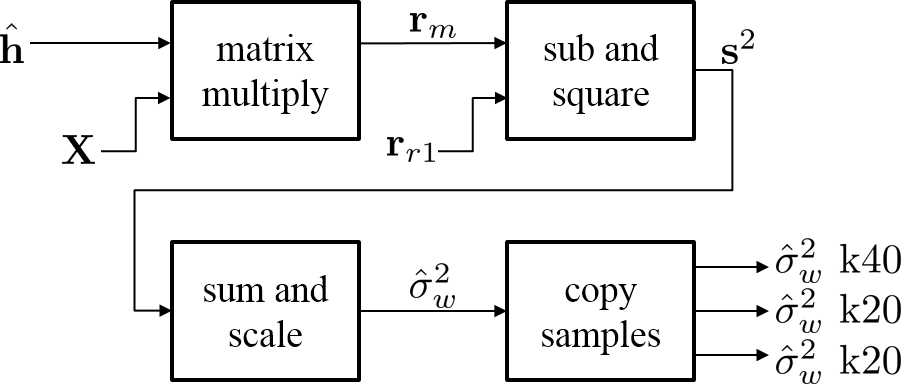
\includegraphics[width=\textwidth/10*8]{figures/gpu/noiseBlock.png}
	\caption{The block diagram for the Noise Variance estimator.}
	\label{fig:noiseBlock}
\end{figure}
With the frequency offset removed and the channel estimated, the noise variance can be estimated.
The noise variance was studied in section \ref{sec:noise-variance} and \ref{sec:joint-ML-estimator}.
Equation \eqref{eq:ML-s2-final3} is the final form of the noise variance estimator and repeated here for convenience.

\begin{equation}
	\hat{\sigma}_w^2 = \frac{1}{2\rho} \left| \mathbf{r}-\hat{\boldsymbol{\Omega}}_0\mathbf{X}\hat{\mathbf{h}}\right|^2
	\label{eq:jeff-ML-s2-final3}
\end{equation}
where
\begin{equation}
	\rho = {\rm Trace} \left\{ \mathbf{I} -  \mathbf{X}\left(\mathbf{X}^\dag\mathbf{X}\right)^{-1}\mathbf{X}^\dag \right\}.
\end{equation}

Once again, $\boldsymbol{\Omega}_0$ is included in \eqref{eq:jeff-ML-s2-final3} assuming the vector $\mathbf{r}$ has a frequency offset.
The vector $\mathbf{r}_{r1}$ are received samples with the frequency offset compensated for, $\mathbf{r}_{r1}$ is the same vector from the channel estimator.
The noise variance estimator is reformulated replacing $\mathbf{r}$ and removing $\boldsymbol{\Omega}_0$.
\begin{equation}
	\hat{\sigma}_w^2 = \frac{1}{2\rho} \left| \mathbf{r}_{r1}-\mathbf{X}\hat{\mathbf{h}}\right|^2.
	\label{eq:noise_var_reformed}
\end{equation}

To begin estimating the noise variance, the GPU first computes the matrix multiplication $\mathbf{X}\hat{\mathbf{h}}$.
The stored matrix $\mathbf{X}$ is a $(L_p+L_a-N_1-N_2)\times (N_1+N_2+1)$ convolution matrix and the channel estimate $\hat{\mathbf{h}}$ is a $(N_1+N_2+1)\times1$ vector.
The result of the matrix product $\mathbf{r}_m$ is simply the ideal preamble distorted by the estimated multipath channel.
The GPU calls a CUBLAS function to compute $\mathbf{r}_m$ quickly and efficiently.

With $\mathbf{r}_m$ computed, $\frac{1}{2\rho} \left| \mathbf{r}_{r1}-\mathbf{r}_m\right|^2$ is split into two GPU kernels.
The first GPU kernel computes $\mathbf{s}^2$, an element by element magnitude squared difference vector of $\mathbf{r}_{m}$ and $\mathbf{r}_{r1}$ with $L_p+L_a-N_1-N_2$ threads for each packet.
\begin{equation}
s^2(n) = \left| r_{r1}(n)- r_m(n) \right|^2
\end{equation}

For each packet, $\hat{\sigma}_w^2$ is computed by scaling the summation of by $\frac{1}{2\rho}$ in one GPU kernel.
The GPU kernel is launched with one thread per packet to scale a summation of $\mathbf{s}^2$ by $\nicefrac{1}{2\rho}$.
$\rho$ is a precomputed scalar based on the convolution matrix $\mathbf{X}$.
With the noise variance estimated for each packet, the estimates are transferred from the k40 GPU to the k20 GPUs.
These kernels are shown in Figure \ref{fig:noiseBlock}.


\subsection{Equalizer GPU Implementation}


\subsubsection{Zero-Forcing Equalizer}
The Zero-Forcing (ZF) equalizer was explored in section \ref{sec:zf}.
Equation \eqref{eq:spike-solution} computes the ZF filter coefficients.
The equation is repeated here for convenience with an added subscript.
\begin{equation}
	\mathbf{c}_{ZF} = \left( \mathbf{H}^\dag\mathbf{H}\right)^{-1}\mathbf{H}^\dag\mathbf{u}_{n_0}
	\label{eq:jeff-spike-solution}
\end{equation}
where $\mathbf{H}$ is the $(N_1+N_2+L_1+L_2+1)\times (L_1+L_2+1)$
convolution matrix formed by the channel impulse response $\hat{\mathbf{h}}$:
\begin{equation}
	\mathbf{H} = \begin{bmatrix}
		\hat{h}(-N_1) 	&  &  & \\
		\hat{h}(-N_1+1) & \hat{h}(-N_1) & & \\
		\vdots & \vdots & \ddots & \\
		\hat{h}(N_2) 	& \hat{h}(N_2-1) & & \hat{h}(-N_1)\\
		       & \hat{h}(N_2) & & \hat{h}(-N_1+1) \\
		       &        & & \vdots \\
		       &        & & \hat{h}(N_2)
		\end{bmatrix}.
\label{eq:jeff-zf-H-matrix}
\end{equation}
The length $L_1+L_2+1$ is the length of the equalizer $L_{eq}$.
The length $N_1+B_2$ is the length of the channel $L_ch$.
and we assume $c(n)$ has support on $-L_1 \leq n \leq L_2$ and that $\hat{h}(n)$
has support on $-N_1 \leq n \leq N_2$.
$\mathbf{u}_{n_0}$ is the $(N_1+N_2+L_1+L_2+1) \times 1$
vector representing the desired composite impulse response:
that is, a vector comprising all-zeros with a one in position $n_0$.
These vectors are
\begin{equation}
	\mathbf{c}_\text{ZF} = \begin{bmatrix} c(-L_1) \\ \vdots \\ c(0) \\ \vdots \\ c(L_2) \end{bmatrix}
	\qquad
	\mathbf{u}_{n_0} = \begin{bmatrix} 0 \\ \vdots \\ 0 \\ 1 \\ 0 \\ \vdots \\ 0 \end{bmatrix}
	\begin{matrix*}[l] \left. \vphantom{\begin{matrix} 0 \\ \vdots \\ 0 \end{matrix}} \right\}
		\text{$n_0-1$ zeros}
		\\ \\
		\left. \vphantom{\begin{matrix} 0 \\ \vdots \\ 0 \end{matrix}} \right\}
		\text{$N_1+N_2+L_1+L_2-n_0+1$ zeros}
		\end{matrix*}
\label{eq:jeff-cu-vector-def}
\end{equation}

In equation \eqref{eq:jeff-spike-solution}, $\mathbf{H}^\dag\mathbf{H}$ is of the form
\begin{equation}
\mathbf{R}_{h_\text{ZF}} = \mathbf{H}^\dag\mathbf{H} = 
	\begin{bmatrix}
		r_{h_\text{ZF}}(0) 				& r_{h_\text{ZF}}(-1) 			& \cdots & r_{h_\text{ZF}}(-L_1-L_2)	\\
		r_{h_\text{ZF}}(1) 		& r_{h_\text{ZF}}(0) 			& \cdots & r_{h_\text{ZF}}(-L_1-L_2+1)		\\
		\vdots 				& \vdots 			& \ddots & \vdots  			\\
		\\
		r_{h_\text{ZF}}(L_1+L_2) & r_{h_\text{ZF}}(L_1+L_2)	& \cdots & r_{h_\text{ZF}}(0)  			\\
	\end{bmatrix}
	\label{eq:hhh}
\end{equation}
where $r_{h_\text{ZF}}(k)$ is the auto-correlation of the estimated channel
\begin{equation}
r_{h_\text{ZF}}(k) = \sum_{n=-N_1}^{N_2} \hat{h}(n)\hat{h}^\ast(n-k).
\end{equation}
The definition of $\mathbf{R}_{h_\text{ZF}}$, requires $r_{h_\text{ZF}}(k)$ for $-L_1-L_2 \leq n \leq L_1+L_2$. 
But $r_{h_\text{ZF}}(k)$ only has support on $-N_1-N_2 \leq n \leq N_1+N_2$ resulting in $r_{h_\text{ZF}}(k)$ being sparse which means $r_{h_\text{ZF}}(k)$ is mostly zero. 
In \eqref{eq:hhh}, $r_{h_\text{ZF}}(k)$ for $\left|k\right| > N_1+N_2$ is zero resulting in $\mathbf{R}_{h_\text{ZF}}$ also being sparse. 
In fact, $\mathbf{R}_{h_\text{ZF}}$ is $\% 64$ zeros.

In equation \eqref{eq:jeff-spike-solution}, $\mathbf{H}^\dag\mathbf{u}_{n_0}$ can be simplified to the vector $\hat{\mathbf{h}}_{n_0}$
\begin{equation}
	\mathbf{H}^\dag\mathbf{u}_{n_0} = \hat{\mathbf{h}}_{n_0} = \begin{bmatrix} 0 \\ \vdots \\ 0 \\ \mathbf{h} \\ 0 \\ \vdots \\ 0 \end{bmatrix}
	\begin{matrix*}[l] \left. \vphantom{\begin{matrix} 0 \\ \vdots \\ 0 \end{matrix}} \right\}
		\text{$n_0-N_1-1$ zeros}
		\\ \\
		\left. \vphantom{\begin{matrix} 0 \\ \vdots \\ 0 \end{matrix}} \right\}
		\text{$N_1+L_1+L_2-n_0+1$ zeros.}
		\end{matrix*}
\label{eq:hun0-vector-def}
\end{equation}
where $\hat{\mathbf{h}}_{n_0}$ is just a zero padded version of the channel estimate $\mathbf{h}$.

\begin{figure}
	\centering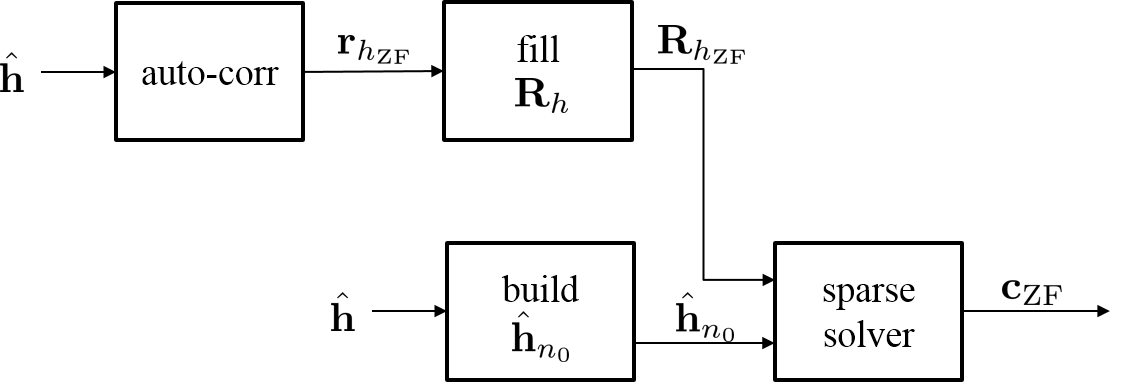
\includegraphics[width=\textwidth/10*8]{figures/gpu/ZFblock.png}
	\caption{The block diagram for the Zero Forcing equalizer implementation.}
	\label{fig:ZFblock}
\end{figure}

The computation of $\mathbf{c}_\text{ZF}$ looks fairly straight forward but the inverse of $\mathbf{H}^\dag\mathbf{H}$ presents a very challenging problem in GPU implementation.
GPUs perform extremely well on parallel algorithms but an inverse is inherently serial.
If the inverse was to implemented, the computation takes longer than $1.9065$ seconds.
Equation \eqref{eq:jeff-spike-solution} must be reformed to remove the inverse of $\mathbf{H}^\dag\mathbf{H}$.
\begin{equation}
	\mathbf{H}^\dag\mathbf{H}\mathbf{c}_\text{ZF} = \mathbf{H}^\dag\mathbf{u}_{n_0}
	\label{eq:jeff-spike-solution-reformed}
\end{equation}
or
\begin{equation}
	\mathbf{R}_{h_\text{ZF}} \mathbf{c}_\text{ZF} = \hat{\mathbf{h}}_{n_0}
	\label{eq:jeff-spike-solution-reformed_vectors}
\end{equation}


To eliminate the need for an inverse, $\mathbf{H}^\dag\mathbf{H}$ is moved to the left side of equation \eqref{eq:jeff-spike-solution}. Solving for $\mathbf{c}_\text{ZF}$ in \eqref{eq:jeff-spike-solution-reformed_vectors} can be done many ways but the sparseness of $\mathbf{R}_{h_\text{ZF}}$ must be leveraged to ensure the coeffiencts can be calcualted with in the $1.9065$ seconds. 
Nvidia has a batched sparse solver library that computes $3103$ $\mathbf{c}_\text{ZF}$ equalizers in less than $410$ms.

Figure \ref{fig:ZFblock} shows the ZF filter calculations only require the channel estimate $\hat{\mathbf{h}}$.
The GPU launches a kernel with $2(N_1+N_2)+1$ threads per packet to calculate the estimated channel auto-correlation $\mathbf{R}_{h_\text{ZF}}$.
The matrix $\mathbf{R}_{h_\text{ZF}}$ is built by the GPU with $\mathbf{R}_{h_\text{ZF}}$ by launching a kernel with a thread for every non-zero index in $\mathbf{R}_{h_\text{ZF}}$.
The GPU also builds the vector $\hat{\mathbf{h}}_{n_0}$ by zero padding the channel estimate with $N_1+N_2+1$ threads per packet.
The Zero forcing equalizer coefficients are then calculated using the batched sparse solver from the CUDA libary.



\clearpage
\subsubsection{MMSE Equalizer}
The general formulation for the MMSE equalizer is the same as ZF equalizer.
The MMSE equalizer was explored in section \ref{sec:mmse}.
Equation \eqref{eq:copt-Ri} computes the MMSE filter coefficients.
The equation is repeated here for convenience with an added subscript.
The MMSE optimum equalizer filter coefficients are given by
\begin{equation}
	\mathbf{c}_\text{MMSE} = \left[ \vphantom{\sum} \mathbf{H}^\dag\mathbf{H} + %\frac{1}{2\nicefrac{E_b}{N_0}}
	\frac{2\sigma^2_w}{\sigma^2_s}
	\mathbf{I}_{L_1+L_2+1} \right]^{-1}
	\mathbf{g}^\dag
	\label{eq:jeff-copt-Ri}
\end{equation}
where $\mathbf{H}$ is the same $\mathbf{H}$ from the ZF equalizer in equation \eqref{eq:jeff-zf-H-matrix} and $\mathbf{I}_{L_1+L_2+1}$ is the $(L_1+L_2+1)\times(L_1+L_2+1)$ identity matrix.
The vector $\mathbf{g}^\dag$ is also the same as the vector $\hat{\mathbf{h}}_{n_0}$ in the ZF equalizer in equation \eqref{eq:hun0-vector-def}.
\begin{figure}
	\centering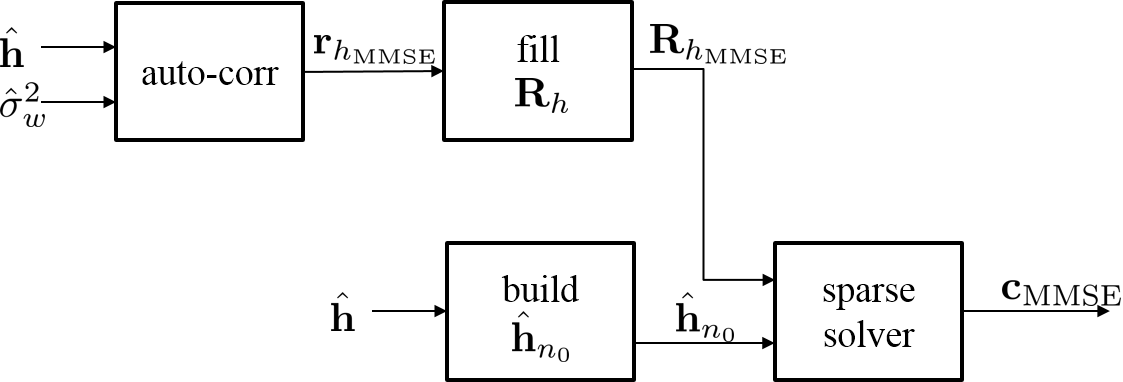
\includegraphics[width=\textwidth/10*8]{figures/gpu/MMSEblock.png}
	\caption{The block diagram for the MMSE equalizer implementation.}
	\label{fig:MMSEblock}
\end{figure}
The matrix operations in \eqref{eq:jeff-copt-Ri} can be expressed as
\begin{equation}
\left[\vphantom{\sum} \mathbf{H}^\dag\mathbf{H} + %\frac{1}{2\nicefrac{E_b}{N_0}}
	\frac{2\sigma^2_w}{\sigma^2_s}
	\mathbf{I}_{L_1+L_2+1}\right] = \mathbf{R}_{h_\text{MMSE}}
\end{equation}
where
\begin{equation}
\mathbf{R}_{h_\text{MMSE}} = 
		\begin{bmatrix}
		r_{h_\text{MMSE}}(0)				 & r_{h_\text{MMSE}}(-1) 			& \cdots & r_{h_\text{MMSE}}(-L_1-L_2)	\\
		r_{h_\text{MMSE}}(1) 		& r_{h_\text{MMSE}}(0)& \cdots & r_{h_\text{MMSE}}(-L_1-L_2+1)		\\
		\vdots 				& \vdots 			& \ddots & \vdots  			\\
		\\
		r_{h_\text{MMSE}}(L_1+L_2) & r_{h_\text{MMSE}}(L_1+L_2)	& \cdots & r_{h_\text{MMSE}}(0)		\\
	\end{bmatrix}
\end{equation}
and
\begin{equation}
r_{h_\text{MMSE}}(k) = \sum_{n=-N_1}^{N_2} \hat{h}(n)\hat{h}^\ast(n-k) + \hat{\sigma}_w^2 \delta(k).
\end{equation}

The MMSE equalizer coeffiencts are calculated almost the same way as the ZF equalizer.
The only little difference is calculating $r_{h_\text{MMSE}}(k)$, the noise variance $\hat{\sigma}_w^2$ is added to $r_{h_\text{MMSE}}(0)$. 
Aside from adding $\hat{\sigma}_w^2$, the GPU implements 
\begin{equation}
	\mathbf{R}_{h_\text{MMSE}} \mathbf{c}_\text{MMSE} = \hat{\mathbf{h}}_{n_0}
	\label{eq:jeff-ZF-vectors}
\end{equation}
exactly the same way as equation \eqref{eq:jeff-spike-solution-reformed_vectors}. 
The MMSE block diagram in Figure \ref{fig:MMSEblock} is the same as the ZF block diagram in Figure \ref{fig:ZFblock} aside from the noise variance going into the auto-corr block.

\subsubsection{CMA Equalizer}
The constant modulus algorithm (CMA) equalizer was explored in section \ref{sec:CMA}.
Equation \eqref{eq:cma-update-summary} updates the CMA filter coefficients using Equation \ref{eq:DelJcma-approx} to compute $\nabla J_\text{CMA}$.
The equations are repeated here for convenience with a few changes.
\begin{equation}
	\nabla J_\text{CMA} \approx \frac{2}{2N_b} \sum_{n=0}^{2N_b-1}
	\left[ \vphantom{\displaystyle\sum}  y(n) y^\ast(n) - R_2 \right]
	y(n)  \mathbf{r}^\ast(n).
\label{eq:jeff-DelJcma-approx}
\end{equation}
\begin{equation}
	\mathbf{c}_{b+1} = \mathbf{c}_b - \mu \nabla J_\text{CMA}
\label{eq:jeff-cma-update-summary}
\end{equation}
In section \ref{sec:CMA} equation \eqref{eq:jeff-DelJcma-approx} was derived generally, but here we now have known data and equalizer lengths.
There is only one $\nabla \mathbf{J}_\text{CMA}$ so the subscript CMA is dropped.
The adjustment $\nabla \mathbf{J}$ is the same length $L_{eq}$ as the equalizer $\mathbf{c}_n$.
The portion of $\mathbf{r}^\ast(k)$ starts at the center tap of the equalizer $L_1$.
The block index does not need to be tracked because of the frame synconization step, so the subscript $b+1$ and $b$ is replaced with the iteration index $n$ and $n+1$.
Because the index $n$ is being used as the iteration index, the summation index is replaced with $k$.
Applying all of these changes results in 
\begin{equation}
	\nabla \mathbf{J} \approx \sum_{k=0}^{L_{pkt}-1} 
	z(k) \mathbf{r}^\ast(k).
\label{eq:jeff-DelJcma-approx}
\end{equation}
\begin{equation}
	\mathbf{c}_{n+1} = \mathbf{c}_n - \mu \nabla \mathbf{J}
\label{eq:jeff-cma-update-summary}
\end{equation}
where
\begin{equation}
z(k) = \left[ \vphantom{\displaystyle\sum}  y(k) y^\ast(k) - R_2 \right]
	y(k).
\end{equation}

The computation of $\nabla \mathbf{J}$ can be done directly by launching $L_{eq}$ threads to compute a length $L_{pkt}$ summation per thread.
But a long summation inside a GPU thread is terribly inefficient.
The equation for $\nabla \mathbf{J}$ can be reformulated or massaged to look like a convolutional sum.
This will be shown by by doing a toy example.

Suppose that the vectors $\mathbf{r}^\ast$ and $\mathbf{z}$ are length $4$ and zero outside of $0 \leq k \leq 3$. 
The desired vector $\nabla \mathbf{J}$ is $3$ long and $L_1$ is $1$.
The toy example computation of $\nabla \mathbf{J}$ is
\begin{align}
\nabla J(0) &= z(0)r(1)				+z(1)r(2) +z(2)r(3)				\\ \nonumber
\nabla J(1) &= z(0)r(0)				+z(1)r(1) +z(2)r(2)	+z(3)r(3)	\\ \nonumber
\nabla J(2) &= \indent\indent\indent\;  z(1)r(0) +z(2)r(1) +z(3)r(2).	\\ \nonumber
\label{eq:toy-delj}
\end{align}
A convolutional sum of the vector $\mathbf{z}$ with $\mathbf{r}$ is
\begin{align}
y(0) &= z(0)r(0)																		\\\nonumber
y(1) &= z(0)r(1) 				+z(1)r(0)													\\ \nonumber
y(2) &= z(0)r(2) 				+z(1)r(1) 				+z(2)r(0)							\\ \nonumber
y(3) &= z(0)r(3) 				+z(1)r(2) 				+z(2)r(1) 				+z(3)r(0) 	\\ \nonumber
y(4) &= \indent\indent\indent\;  z(1)r(3) 				+z(2)r(2) 				+z(3)r(1) \\ \nonumber
y(5) &= \indent\indent\indent\indent\indent\indent\>\,\, z(2)r(3) 				+z(3)r(2) \\ \nonumber
y(6) &= \indent\indent\indent\indent\indent\indent\indent\indent\indent\;\;\;		 z(3)r(3) \\ \nonumber
\label{eq:toy-conv}
\end{align}
The convolutional sum looks kind of like the $\nabla \mathbf{J}$ but longer.
The desired section of $\mathbf{y}$ is $2 \leq k \leq 4$.
\begin{align}
y(2) &= z(0)r(2) 				+z(1)r(1) 				+z(2)r(0)							\\ \nonumber
y(3) &= z(0)r(3) 				+z(1)r(2) 				+z(2)r(1) 				+z(3)r(0) 	\\ \nonumber
y(4) &= \indent\indent\indent\;  z(1)r(3) 				+z(2)r(2) 				+z(3)r(1)  \nonumber
\label{eq:y_portion}
\end{align}
The set of convolutional equations are structured like $\nabla \mathbf{J}$ but the indices in $r(n)$ are ascending in Equations \eqref{eq:toy-delj} but descending in Equations \eqref{eq:y_portion}.
One of the input vectors $\mathbf{z}$ or $\mathbf{r}$ need to be reversed.

\clearpage
Now the indicies are moving in the right directions but the convolutional sum has the wrong structure.
The vector $\mathbf{y}$ needs to be reversed also.
\begin{align}
y(4) &= z(0)r(1)				+z(1)r(2) +z(2)r(3)				\\ \nonumber
y(3) &= z(0)r(0)				+z(1)r(1) +z(2)r(2)	+z(3)r(3)	\\ \nonumber
y(2) &= \indent\indent\indent\;  z(1)r(0) +z(2)r(1) +z(3)r(2).	\\ \nonumber
\label{eq:y_reverse}
\end{align}
Now the convolutional sum $\mathbf{y}$ has been massaged to look just like $\nabla \mathbf{J}$.
\begin{align}
\nabla J(0) &= z(0)r(1)				+z(1)r(2) +z(2)r(3)				\\ \nonumber
\nabla J(1) &= z(0)r(0)				+z(1)r(1) +z(2)r(2)	+z(3)r(3)	\\ \nonumber
\nabla J(2) &= \indent\indent\indent\;  z(1)r(0) +z(2)r(1) +z(3)r(2).	\\ \nonumber
\label{eq:toy-delj_repeat}
\end{align}

This Toy example shows that a simple convolution can be used to calculate $\nabla \mathbf{J}$ instead of a long summation for each index of the gradient.
Figure \ref{fig:delJ_convORsum} shows how to use a convolution to compute $\nabla \mathbf{J}$.
One of the input vectors and the output vector must be reversed to compute $\nabla \mathbf{J}$ using a convolution.
The $L_{eq}$ long portion of the convolution starts at the index $L_{pkt} - L_2 - 1$.
\begin{figure}
	\centering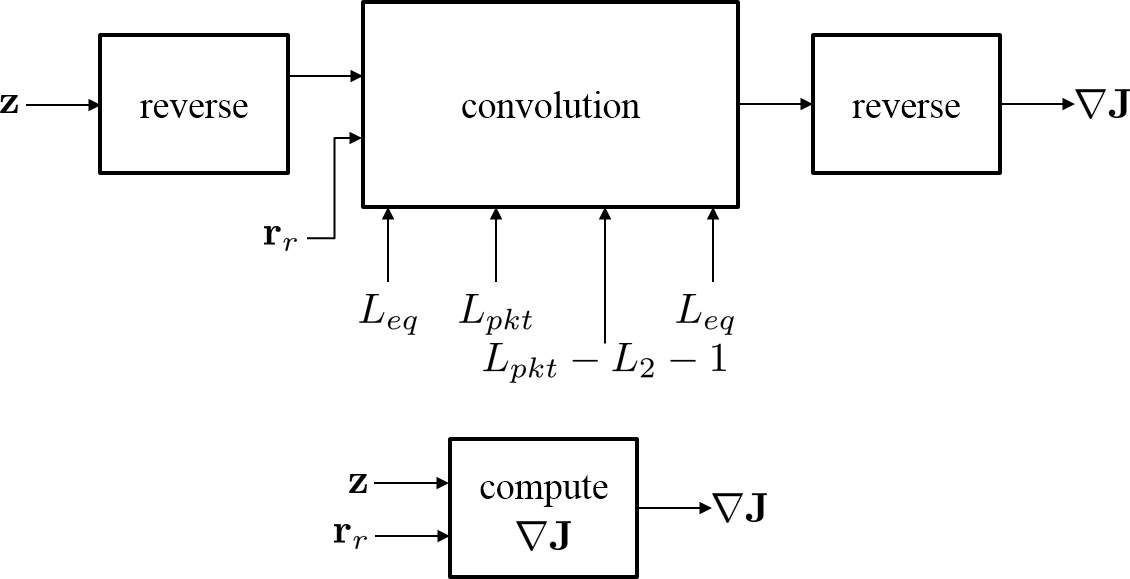
\includegraphics[width=\textwidth/10*8]{figures/gpu/delJ_convORsum.png}
	\caption{The computation of $\nabla \mathbf{J}$ can be done with a convolution of directly.}
	\label{fig:delJ_convORsum}
\end{figure}
The block diagram in Figure \ref{fig:CMA_block} shows how the GPU implements the CMA algorithm.
First the past filter $\mathbf{c}_n$ is applied by a convolution.
The GPU computes $\mathbf{z}$ using $L_{pkt}$ threads per packet, then reverses the vector in preparation for the convolution.
The convolution is done as shown in Figure \ref{fig:conv_FFT_block}.
The GPU then reverses the output vector to obtain $\nabla \mathbf{J}$ from the convolution.
With $\nabla \mathbf{J}$ computed, the next CMA filter coefficients $\mathbf{c}_{n+1}$ are updated using $L_{eq}$ threads per packet.
\begin{figure}
	\centering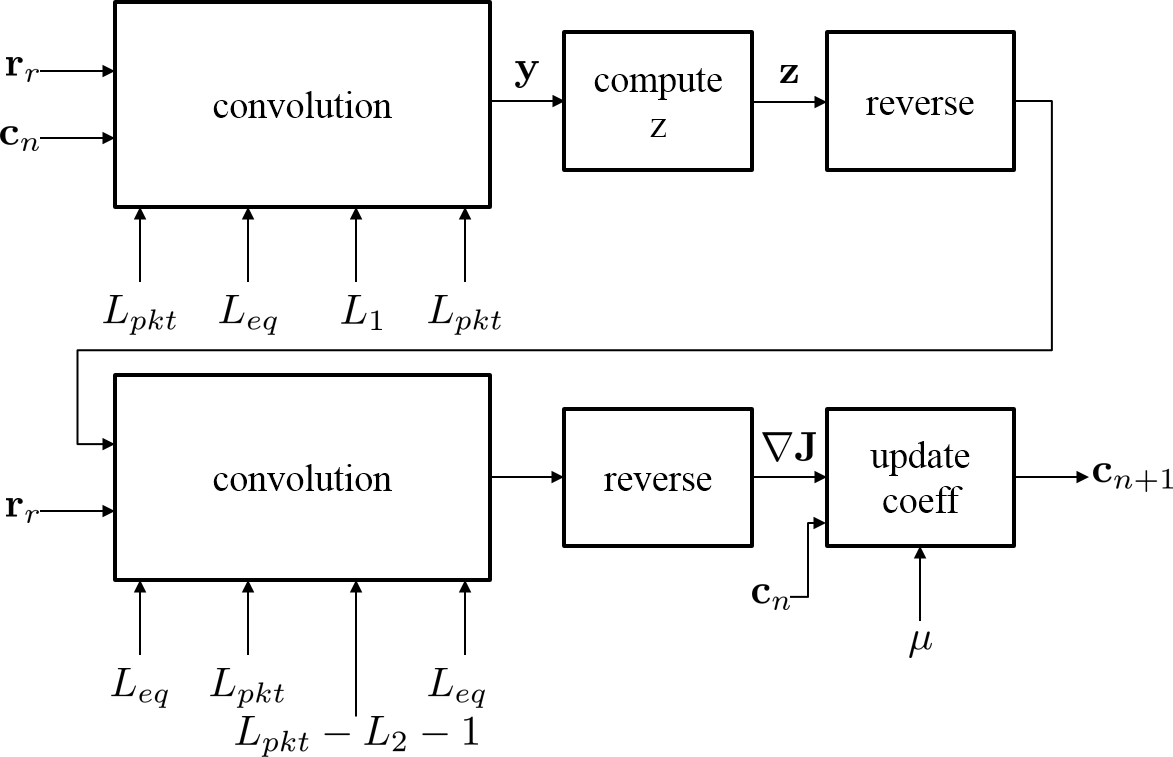
\includegraphics[width=\textwidth/10*8]{figures/gpu/CMA_block.png}
	\caption{The block diagram showing how the GPU implements the CMA algorithm.}
	\label{fig:CMA_block}
\end{figure}


\subsubsection{Frequency Domain Equalizer 1}
The Frequency Domain Equalizer 1 (FDE1) was studied in section....
Equation .... is the final form of the equalizer.
This equation is repeated here
\begin{equation}
\text{FDE}_1 = \frac{\mathbf{H}^*}{\|\mathbf{H}\|^2 + \sigma_0^2}
\label{eq:FDE1}
\end{equation}
Equation \eqref{eq:FDE1} is extremely easy to implement in the GPU.
All that is need to calculate the equalizer is the Fourier Transform of $\hat{\mathbf{h}}$ and the noise variance $\sigma_0^2$.
As shown in Figure \ref{fig:FDE1_block}, the GPU zero pads that channel estimate then takes the $N_{FFT}$ point FFT to obtain $\mathbf{H}$.
Equation \eqref{eq:FDE1} is then calculated by launching $N_{FFT}$ threads per packet.
The output of the multiply $\text{FDE}_1$ is the Frequency Domain Equalizer left in the  frequency domain.
\begin{figure}
	\centering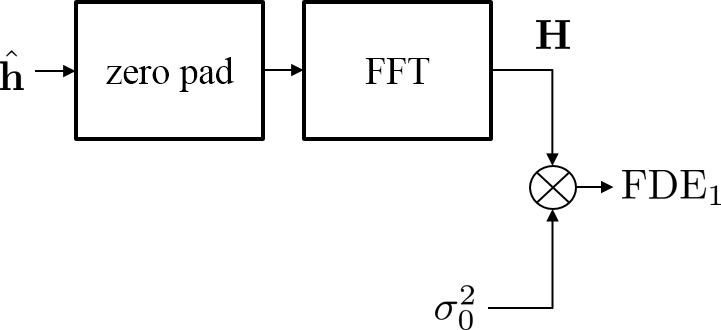
\includegraphics[width=\textwidth/10*5]{figures/gpu/FDE1_block.png}
	\caption{The block diagram showing how the GPU calculates the $\text{FDE}_1$ equalizer.}
	\label{fig:FDE1_block}
\end{figure}

\subsubsection{Frequency Domain Equalizer 2}
The Frequency Domain Equalizer 2 (FDE2) was studied in section....
Equation .... is the final form of the equalizer.
$\text{FDE}_2$ is very simmilar to $\text{FDE}_1$, $\text{FDE}_2$ has an extra term on $\sigma_0^2$
This equation is repeated here
\begin{equation}
\text{FDE}_2 = \frac{\mathbf{H}^*}{\|\mathbf{H}\|^2 + \sigma_0^2 \mathbf{\Psi}}
\label{eq:FDE2}
\end{equation}
Equation \eqref{eq:FDE2} is implemented the same way \eqref{eq:FDE1} but $\text{FDE}_2$ has one extra vector $\mathbf{\Psi}$ in the multiply.
The vector $\mathbf{\Psi}$ is recomputed and stored.
The output of the multiply $\text{FDE}_2$ is the Frequency Domain Equalizer left in the  frequency domain.
\begin{figure}
	\centering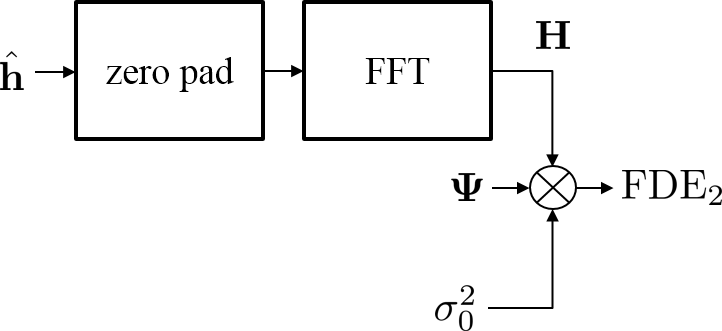
\includegraphics[width=\textwidth/10*5]{figures/gpu/FDE2_block.png}
	\caption{The block diagram showing how the GPU calculates the $\text{FDE}_2$ equalizer.}
	\label{fig:FDE2_block}
\end{figure}

\subsection{Filter Application GPU Implementation}
With all the equalizers calculated and ready to apply, the GPU applys the FIR equalizers and the Numerically Optimized detection filter \cite{NO_perrins}.
The Perrins detection filter length $L_{df}$ is 21 samples long with the center tap at index 10.

\subsubsection{FIR Equalizer Application}
The FIR equalizers (ZF, MMSE and CMA) and the Perrins detection filter are all applied using the convolution block shown in Figure \ref{fig:conv_FFT_block3} and \ref{fig:conv_simple_block}.
\begin{figure}
	\centering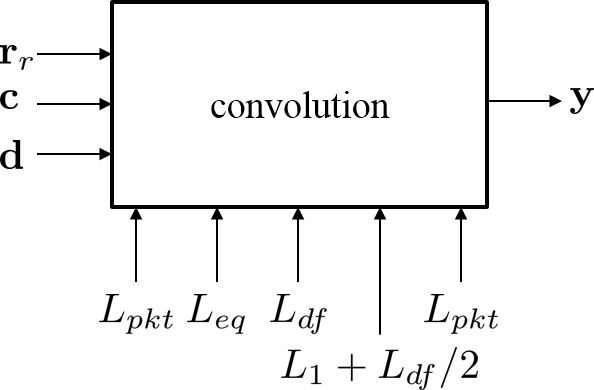
\includegraphics[width=\textwidth/10*5]{figures/gpu/apply_FIR_equalizer.png}
	\caption{The block diagram showing how the GPU applies an FIR equlizer and the Numerically Optimized Perrins detection filter.}
	\label{fig:apply_FIR_equalizer}
\end{figure}
The derotated samples vector $\mathbf{r}_r$ is $L_{pkt}$ or $12672$ samples long.
The calculated equalizer $\mathbf{c}$ is $L_{eq}$ or $186$ samples long.
The Perrins Numerically Optimized detection filter $\mathbf{d}$ is $L_{df}$ or $21$ samples long.
The $L_{pkt}$ samples that need to be pruned out start at $L_1+L_{df}/2$.
The vector $\mathbf{y}$ are samples that have been equalized and detected, ready for the symbol detector and Phase Lock Loop.

\clearpage
\subsubsection{Frequency Domain Equalizer Application}
The application of the Frequency Domain Equalizers, $\text{FDE}_1$ and $\text{FDE}_2$, are not applied using the conventional convolution.
$\text{FDE}_1$ and $\text{FDE}_2$ are applied in the frequency domain by
\begin{equation}
\text{FDE}_2 = \frac{\mathbf{H}^*\mathbf{R}_r \mathbf{D}}{\|\mathbf{H}\|^2 + \sigma_0^2}
\label{eq:apply_FDE1}
\end{equation}
and
\begin{equation}
\text{FDE}_2 = \frac{\mathbf{H}^*\mathbf{R}_r \mathbf{D}}{\|\mathbf{H}\|^2 + \sigma_0^2 \mathbf{\Psi}}
\label{eq:apply_FDE2}
\end{equation}
where $\mathbf{R}_r$ is the Fourier transform of the zero padded derotated samples $\mathbf{r}_r$ and $\mathbf{D}$ is the Fourier transform of the zero padded detection filter $\mathbf{d}$.
The Fourier transform of Perrins Detection filter was initialized and stored.

Figures \ref{fig:apply_FDE1} and \ref{fig:apply_FDE2} show block diagrams of how $\text{FDE}_1$ and $\text{FDE}_2$ is implemented in the GPU.
The vector $\mathbf{\Psi}$ was precomputed and stored at initialization.
The multiply in each figure is not a typical multiplication, the multiply block implements Equations \eqref{eq:FDE1} and \eqref{eq:FDE2}.
To prepare the data for the OQPSK demodulator and Phase Lock Loop, the prune block shown in both figures down samples by 2.
With the signal downsampled to 1 sample per bit, the equalized received signal is ready for the demodulator, Phase Lock Loop and bit decisions.
\begin{figure}
	\centering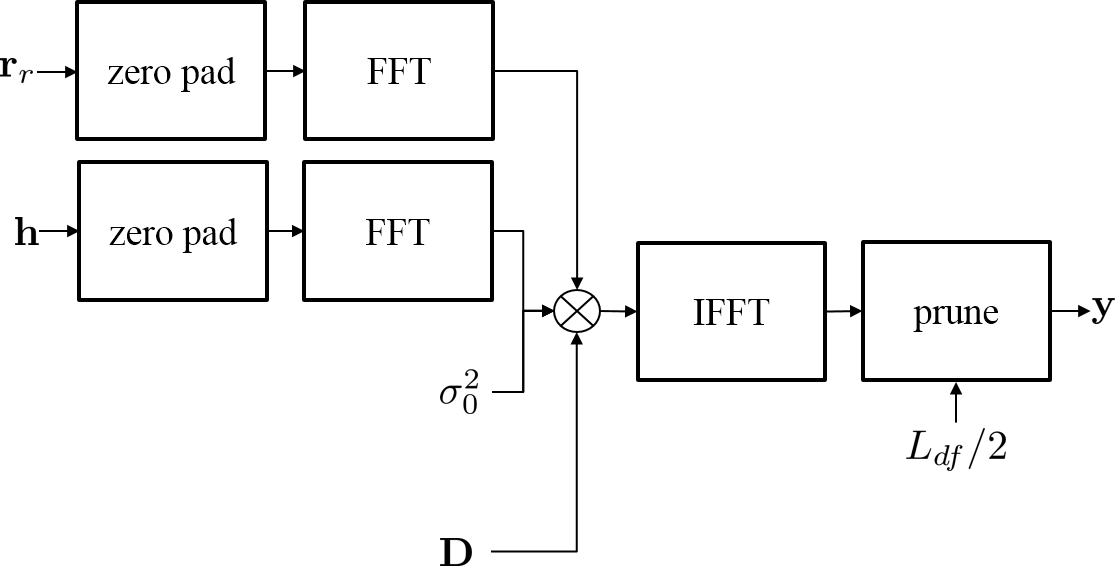
\includegraphics[width=\textwidth/10*8]{figures/gpu/apply_FDE1.png}
	\caption{The block diagram showing how the GPU applies $\text{FDE}_1$ and the Numerically Optimized Perrins detection filter.}
	\label{fig:apply_FDE1}
\end{figure}
\begin{figure}
	\centering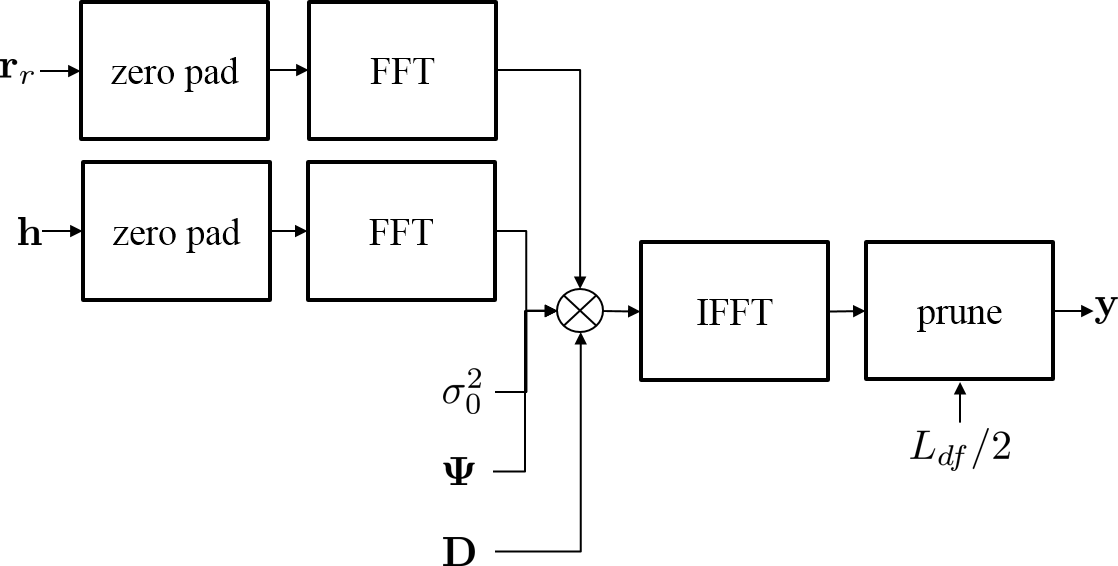
\includegraphics[width=\textwidth/10*8]{figures/gpu/apply_FDE2.png}
	\caption{The block diagram showing how the GPU applies $\text{FDE}_2$ with $\mathbf{\Psi}$ and the Numerically Optimized Perrins detection filter.}
	\label{fig:apply_FDE2}
\end{figure}

\clearpage
\subsection{GPU OQPSK Demodulator Implementation}
After all the equalizers and detection filters have been applied to the received samples there is 5 different streams of equalized samples.
The bit decisions from each stream of equalized samples needs to be obtained.

The top of Figure \ref{fig:demod_block} shows a block diagram of how the bit decisions are made.
A "symbol-by-symbol" OQPSK detector is used to build the data decision vector $\hat{\mathbf{a}}$ for each stream of equalized samples.
The OQPSK detector is first data-aided then decision directed. 
In case the frequency offset estimator in section \ref{sec:jeffs_frequencyoffsetestimator} was imperfect, a first order  with a Phase Lock Loop (PLL) is applied to track out the residual frequency offset.
Figure \ref{fig:demod_loop} shows a block diagram of a first order PLL.

Traditionally a single PLL would be applied to the whole stream of equalized samples because PLLs are inherently serial, but the equalized samples have a packet structure with known data.
A PLL can be applied to each packet introducing parallelism to map best to GPUs.
One thread per packet per stream of equalized samples is launched to run the OQPSK demodulator shown in Figure \ref{fig:demod_loop}.

Starting at the in the preamble of each packet, the PLL tracks out the a frequency offset for $0\leq k \leq L_{pkt}$ by estimating the maximum likelihood phase error $e(k)$ where
\begin{equation*}
e(k)
= 
\begin{cases}
0 &\text{$k$ even} \\
\hat{a}(k-1)\mathbb{I}\{y_r(k-1)\} -  \hat{a}(k)\mathbb{R}\{y_r(k)\}  &\text{$k$ odd}\\
\end{cases}.
\end{equation*}
With the estimated phase error estimated, the gain $K_1$ is applied to $e(k)$ and a Direct Digital Synthesizer (DDS) generates a signal to derotate the equalized sample at index $k$.
For every $y(k)$ in the packet, a derotated sample $y_r(k)$ is calculated and the data decision $\hat{a}(k)$ is estimated where
\begin{equation}
\hat{a}(k)= \begin{cases}
p(k) &k<L_p+L_{asm} \\
sgn(\mathbb{R}\{y_{r}(k)\})&k\geq L_p+L_{asm} \quad \& \quad \text{$k$ even}\\
sgn(\mathbb{I}\{y_{r}(k)\})&k\geq L_p+L_{asm} \quad \& \quad \text{$k$ odd}\\
\end{cases}.
\end{equation}
and $p(k)$ are the known bits or decisions in the preamble and ASM.
Once the index $k$ is out of the preamble and asm, the data decisions $\hat{a}(k)$ are based on the sign of the real $\mathbb{R}$ or imaginary $\mathbb{I}$part of $y_r(k)$. 
\begin{figure}
	\centering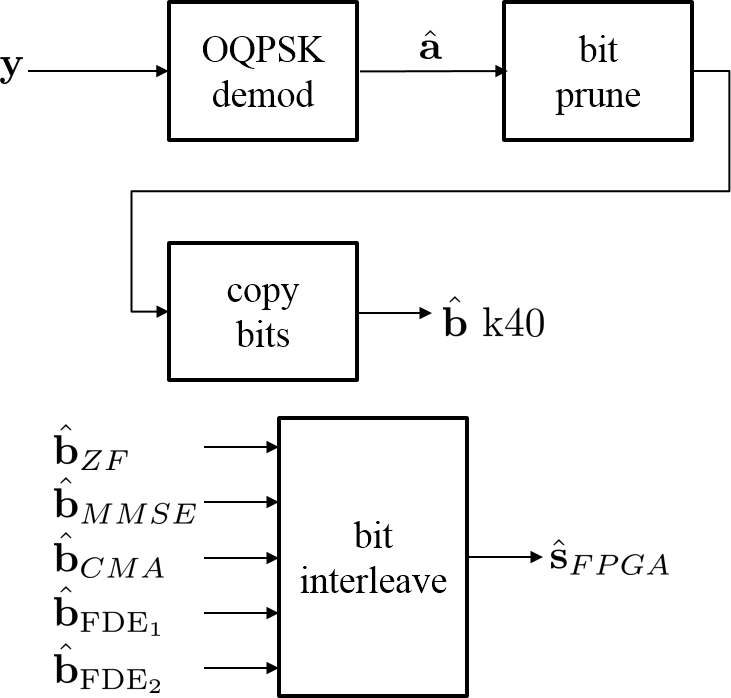
\includegraphics[width=\textwidth/10*5]{figures/gpu/demod_block.png}
	\caption{The block diagram showing how the GPU applies the demodulator to equalized received samples to obtain the bit decisions.}
	\label{fig:demod_block}
\end{figure}
\begin{figure}
	\centering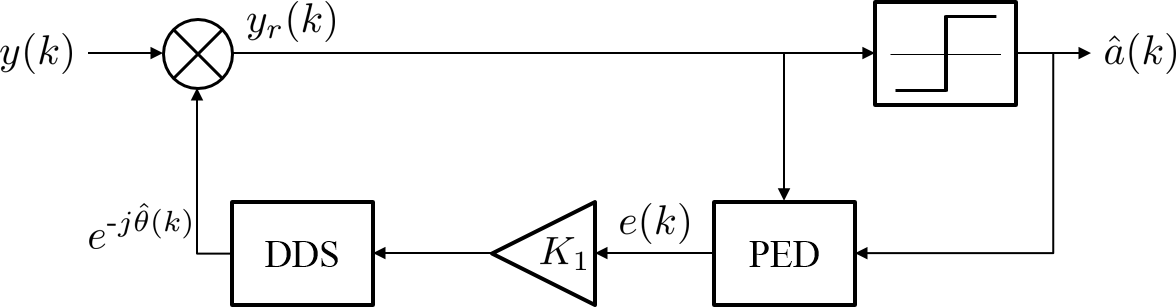
\includegraphics[width=\textwidth/10*8]{figures/gpu/demod_loop.png}
	\caption{The block diagram showing the OQPSK demodulator from Figure \ref{fig:demod_block}. The $\hat{a}(k)$ is data-aided for $k<L_p+L_{asm}$ and decision directed when $k\geq L_p+L_{asm}$.}
	\label{fig:demod_loop}
\end{figure}

After the vector $\hat{\mathbf{a}}$ is calculated, the data bits are pruned out of every packet as shown in Figure \ref{fig:demod_block} as the bit prune block.
One thread per data bit is launched to strip the data bits and build the bit decision vector $\hat{\mathbf{b}}$ from $\hat{\mathbf{a}}$ where
\begin{equation}
\hat{b}(n)
= 
\begin{cases}
0 &\hat{a}(n)>0 \\
1 &\hat{a}(n)<0\\
\end{cases}.
\end{equation}
After the data bit vector $\hat{\mathbf{b}}$ for each equalized stream is built, the bit decisions are all transferred to the Tesla k40 GPU in the copy bits block.
The bit vector $\hat{\mathbf{s}}_{FPGA}$ is a c++ char array containing interleaved bit streams $\hat{\mathbf{b}}$ from each stream of equalized samples. 
In each char index of $\hat{\mathbf{s}}_{FPGA}$ contains 8 bit decisions for a single equalized bit stream.
The first bit stream in $\hat{\mathbf{s}}_{FPGA}$ is the bit stream from the ZF equalizer, followed by MMSE, CMA, $\text{FDE}_1$, $\text{FDE}_2$ then 3 blank streams.
Figure \ref{fig:bit_inter} shows how the pattern repeats every 8 indices in the char array $\hat{\mathbf{s}}_{FPGA}$.
This array $\hat{\mathbf{s}}_{FPGA}$ containing bit decisions from each equalizer is burst into the FPGA then clocked out to the Bit Error Rate Tester.
\begin{figure}
	\centering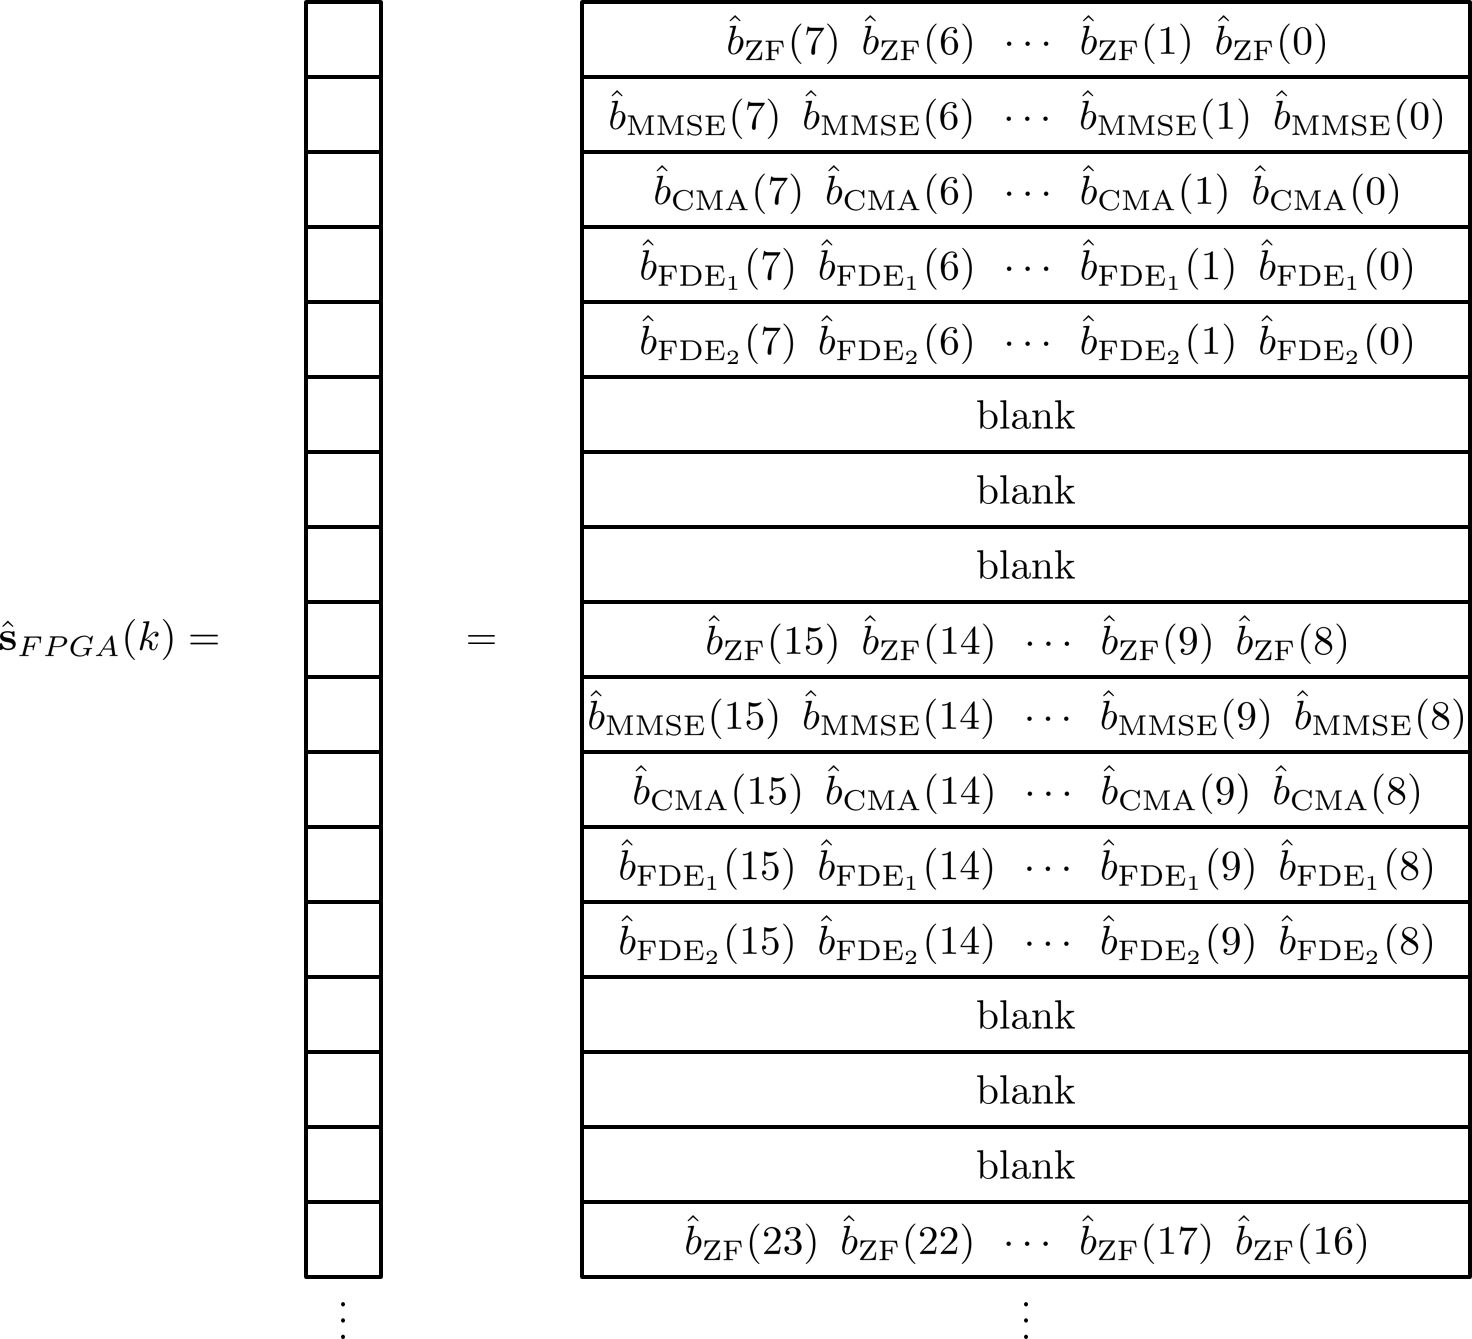
\includegraphics[width=\textwidth/10*8]{figures/gpu/bit_inter.png}
	\caption{The bit stream vector $\hat{\mathbf{s}}_{FPGA}$ is array chars. The bit streams are interleaved and each char contains 8 bit decisions from a single bit stream.}
	\label{fig:bit_inter}
\end{figure}
 
%%%%%%%%%%%%%%%%%%%%%%%%%%%%%%%%%%%%%%%%%%%%%%%%%%%%%%%%%%%%%%%%%%%%%%%%%%%%%%%%%%%%%%%%%%%%%%
%%%%%%%%%%%%%%%%%%%%%%%%%%%%%%%%%%%%%%%%%%%%%%%%%%%%%%%%%%%%%%%%%%%%%%%%%%%%%%%%%%%%%%%%%%%%%%
%%%%%%%%%%% GPU
%%%%%%%%%%%%%%%%%%%%%%%%%%%%%%%%%%%%%%%%%%%%%%%%%%%%%%%%%%%%%%%%%%%%%%%%%%%%%%%%%%%%%%%%%%%%%%
%%%%%%%%%%%%%%%%%%%%%%%%%%%%%%%%%%%%%%%%%%%%%%%%%%%%%%%%%%%%%%%%%%%%%%%%%%%%%%%%%%%%%%%%%%%%%%

% \cleardoublepage
\chapter{Equalizer Equations}
\label{chap:eq_eq}

\section{Overview}
This thesis examines that performance and GPU implementation of 5 equalizers.
While the performance and GPU implementation is interesting, this thesis makes no claim of theoretically expanding understanding of equalizers.
The data-aided equalizers studied in this thesis are:
\begin{itemize}
\item Zero-Forcing (ZF)
\item Minimum Mean Square Error (MMSE)
\item Constant Modulus Algorithm (CMA)
\item Frequency Domain Equalizer 1 (FDE1)
\item Frequency Domain Equalizer 2 (FDE2)
\end{itemize}

The ZF and MMSE equalizers are very similar in formulation though from different sources.
As you might tell from the names, FDE1 and FDE2 are very similar also with one subtle difference.
CMA isn't related to any other algorithm aside from being initialized to MMSE.

\section{Zero-Forcing and Minimum Mean Square Error Equalizers}

The ZF and MMSE equalizers are treated together here because they have many common features.
Both equalizers are found by solving linear equations
\begin{equation}
\mathbf{R}\mathbf{c} = \hat{\mathbf{h}}
\end{equation}
where $\mathbf{c}$ is vector of the desired equalizer coefficients
and $\mathbf{R}$ is the auto-correlation matrix of the channel estimate $\hat{\mathbf{h}}$.
It will be shown that the only difference between ZF and MMSE lies in the the auto-correlation matrix $\mathbf{R}$.

\subsection{Zero-Forcing}
The ZF equalizer is an FIR filter defined by the coefficients
\begin{equation}
\begin{matrix}
c_\text{ZF}(-L_1) & \cdots & c_\text{ZF}(0) & \cdots & c_\text{ZF}(L_2).
\end{matrix}
\end{equation}
The filter coefficients are the solution to the matrix vector equation \cite[eq. (311)]{PAQ-phase1}
\begin{equation}
\mathbf{c}_\text{ZF} = \big(\mathbf{H}^\dagger\mathbf{H}\big)^{-1} \mathbf{H}^\dagger \mathbf{u}_{n_0}
\label{eq:c_ZF_direct}
\end{equation}
where
\begin{equation}
\mathbf{c}_\text{ZF} = 
\begin{bmatrix}
c_\text{ZF}(-L_1) \\ \vdots \\ c_\text{ZF}(0) \\ \vdots \\ c_\text{ZF}(L_2)
\end{bmatrix},
\end{equation}
\begin{equation}
\mathbf{u}_{n_0} = \begin{bmatrix} 0 \\ \vdots \\ 0 \\ 1 \\ 0 \\ \vdots \\ 0 \end{bmatrix}
	\begin{matrix*}[l] \left. \vphantom{\begin{matrix} 0 \\ \vdots \\ 0 \end{matrix}} \right\}
		\text{$n_0-1$ zeros}
		\\ \\
		\left. \vphantom{\begin{matrix} 0 \\ \vdots \\ 0 \end{matrix}} \right\}
		\text{$N_1+N_2+L_1+L_2-n_0+1$ zeros}
		\end{matrix*},
		\label{eq:un0_ZF}
\end{equation}
and
\begin{equation} 
\mathbf{H} = 
		\begin{bmatrix}
		\hat{h}(-N_1)		&  				& 		 	&  					\\
		\hat{h}(-N_1+1) 	& \hat{h}(-N_1)	& 		 	&  					\\
		\vdots	 			& \vdots		& \ddots 	&  					\\
		\hat{h}(N_2)		& \hat{h}(N_2-1)&  			& \hat{h}(-N_1)  	\\
		 					& \hat{h}(N_2) 	&  			& \hat{h}(-N_1+1) 	\\
		 					&  	   			&  			& \vdots			\\
		 					&  	   			&  			& \hat{h}(N_2)		\\
	\end{bmatrix}.
\end{equation}

Calculating Equation \eqref{eq:c_ZF_direct} would give the desired result but the computation is heavy.
The heaviest computation is the $\mathcal{O}(n^3)$ inverse operation followed by the $\mathcal{O}(n^2)$ matrix matrix multiplies.
Rather than performing a heavy inverse, multiplying $\mathbf{H}^\dagger \mathbf{H}$ on both sides of equation \eqref{eq:c_ZF_direct} results in
\begin{align}
\mathbf{H}^\dagger\mathbf{H} \mathbf{c}_\text{ZF} &= \mathbf{H}^\dagger \mathbf{u}_{n_0} \nonumber \\
\mathbf{R}_{\hat{h}} \mathbf{c}_\text{ZF} &= \hat{\mathbf{h}}_{n_0}
\label{eq:c_ZF_solve}
\end{align}
where
\begin{equation}
\mathbf{R}_{\hat{h}} = 
\mathbf{H}^\dagger \mathbf{H} = 
		\begin{bmatrix}
		r_{\hat{h}}(0)			& r^\ast_{\hat{h}}(1)	& \cdots 	& r^\ast_{\hat{h}}(L_{eq}-1)  	\\
		r_{\hat{h}}(1) 			& r_{\hat{h}}(0)		& \cdots 	& r^\ast_{\hat{h}}(L_{eq}-2)  	\\
		\vdots	 				& \vdots				& \ddots 	&  								\\
		r_{\hat{h}}(L_{eq}-1)	& r_{\hat{h}}(L_{eq}-2)	& \cdots	& r_{\hat{h}}(0)  			
	\end{bmatrix}
	\label{eq:R_h}
\end{equation}
is the auto-correlation matrix of the channel estimate $\hat{\mathbf{h}}$ with 
\begin{equation}
r_{\hat{h}}(k) = \sum_{n=-N_1}^{N_2} \hat{h}(n) \hat{h}^\ast(n-k).
\end{equation}
and 
\begin{equation}
\hat{\mathbf{h}}_{n_0} = \mathbf{H}^\dagger \mathbf{u}_{n_0} = 
\begin{bmatrix} \hat{h}^\ast(L_1) \\ \vdots \\ \hat{h}^\ast(0) \\ \vdots \\ \hat{h}^\ast(-L_2)  \end{bmatrix}
\label{eq:h_no}
\end{equation}
is a vector with the time reversed and conjugated channel estimate $\hat{\mathbf{h}}$ centered at $n_0$.

Note that $\mathbf{R}_{\hat{h}}$ can be built by computing
\begin{equation}
\mathbf{r}_{\hat{h}} = 
\begin{bmatrix} r_{\hat{h}}(0) \\ \vdots \\ r_{\hat{h}}(L_{ch}) \\ r_{\hat{h}}(L_{ch}+1) \\ \vdots \\ r_{\hat{h}}(L_{eq}-1)\end{bmatrix} =
\begin{bmatrix} r_{\hat{h}}(0) \\ \vdots \\ r_{\hat{h}}(L_{ch}) \\ 0 \\ \vdots \\ 0  \end{bmatrix},
\end{equation} 
eliminating the need for matrix matrix multiply of $\mathbf{H}^\dagger\mathbf{H}$.
Also, $r_{\hat{h}}(k)$ only has support on $-L_{ch} \leq k \leq L_{ch}$ making $\mathbf{R}_{\hat{h}}$ sparse or $\%63$ zeros.
The sparseness of $\mathbf{R}_{\hat{h}}$ can be leveraged to reduce computation drastically.

%Jeff explains how CUDA solvers handle this equation.
%
%The ZF equalizer was studied in the PAQ Phase 1 Final Report in ~equation 324
%\begin{equation}
%\mathbf{c}_\text{ZF} = (\mathbf{H}^\dagger \mathbf{H})^{-1} \mathbf{H}^\dagger \mathbf{u}_{n_0}
%\label{eq:c_ZF_pinv}
%\end{equation}
%where $\mathbf{c}_\text{ZF}$ is a $L_{eq} \times 1$ vector of equalizer coefficients computed to invert the channel estimate $\hat{\mathbf{h}}$
%and $\mathbf{u}_{n_0}$ is the desired channel impulse response centered on $n0 = N_1+L_1+1$
%\begin{equation}
%\mathbf{u}_{n_0} = \begin{bmatrix} 0 \\ \vdots \\ 0 \\ 1 \\ 0 \\ \vdots \\ 0 \end{bmatrix}
%	\begin{matrix*}[l] \left. \vphantom{\begin{matrix} 0 \\ \vdots \\ 0 \end{matrix}} \right\}
%		\text{$n_0-1$ zeros}
%		\\ \\
%		\left. \vphantom{\begin{matrix} 0 \\ \vdots \\ 0 \end{matrix}} \right\}
%		\text{$N_1+N_2+L_1+L_2-n_0+1$ zeros}
%		\end{matrix*}.
%		\label{eq:un0_ZF}
%\end{equation}
%The $L_{eq}+N_1+N_2 \times L_{eq}$ convolution matrix $\mathbf{H}$ is built using the channel estimate $\hat{\mathbf{h}}$
%\begin{equation}
%\mathbf{H} = 
%		\begin{bmatrix}
%		h(-N_1)		&  			& 		 	&  			\\
%		h(-N_1+1) 	& h(-N_1)	& 		 	&  			\\
%		\vdots	 	& \vdots	& \ddots 	&  			\\
%		h(N_2)		& h(N_2-1) 	&  			& h(-N_1)  	\\
%		 			& h(N_2) 	&  			& h(-N_1+1) \\
%		 			&  	   		&  			& \vdots	\\
%		 			&  	   		&  			& h(N_2)	\\
%	\end{bmatrix}.
%\end{equation}
%The computation of the coefficients in Equation \eqref{eq:c_ZF_pinv} can be simplified in a couple of ways: First the matrix multiplication of $\mathbf{H}^\dagger$ and $\mathbf{H}$ is the autocorrelation matrix of the channel
%\begin{equation}
%\mathbf{R}_{\hat{h}} = 
%\mathbf{H}^\dagger \mathbf{H} = 
%		\begin{bmatrix}
%		r_{h}(0)		& r^\ast_{h}(1)	& \cdots 	& r^\ast_{h}(L_{eq}-1)  	\\
%		r_{h}(1) 		& r_{h}(0)		& \cdots 	& r^\ast_{h}(L_{eq}-2)  	\\
%		\vdots	 			& \vdots				& \ddots 	&  							\\
%		r_{h}(L_{eq}-1)	& r_{h}(L_{eq}-2)	& \cdots	& r_{h}(0)  			
%	\end{bmatrix}
%	\label{eq:R_h}
%\end{equation}
%where
%\begin{equation}
%r_{h}(k) = \sum_{n=-N_1}^{N_2} h(n) h^\ast(n-k).
%\end{equation}
%Second the matrix vector multiplication of $\mathbf{H}^\dagger$ and $\mathbf{u}_{n_0}$ is simply the $n_0$th row of $\mathbf{H}^\dagger$ or the conjugated $n_0$th column of $\mathbf{H}$.
%A new vector $\hat{\mathbf{h}}_{n_0}$ is defined by
%\begin{equation}
%\hat{\mathbf{h}}_{n_0} = \mathbf{H}^\dagger \mathbf{u}_{n_0} = 
%\begin{bmatrix} h(L_1) \\ \vdots \\ h(0) \\ \vdots \\ h(-L_2)  \end{bmatrix}.
%\label{eq:h_no}
%\end{equation}
%To simplify, Equations \eqref{eq:R_h} and \eqref{eq:h_no} are substituted into Equation \eqref{eq:c_ZF_pinv} resulting in 
%\begin{equation}
%\mathbf{c}_\text{ZF} = \mathbf{R}^{-1}_{h} \hat{\mathbf{h}}_{n_0}.
%\label{eq:c_ZF_R_h}
%\end{equation}
%
%Computing the inverse of $\mathbf{R}_{\hat{h}}$ is computationally heavy because an inverse is an $N^3$ operation.
%To avoid an inverse, $\mathbf{R}_{\hat{h}}$ is moved to the left side and $\mathbf{c}_\text{ZF}$ is found by solving a system of linear equations. 
%Note that $r_{h}(k)$ only has support on $-L_{ch} \leq k \leq L_{ch}$ making $\mathbf{R}_{\hat{h}}$ sparse or $\%63$ zeros.
%The sparseness of $\mathbf{R}_{\hat{h}}$ is leveraged to reduce computation drastically.
%The Zero-Forcing Equalizer coefficients are computed by solving
%\begin{equation}
%\mathbf{R}_{\hat{h}} \mathbf{c}_\text{ZF} = \hat{\mathbf{h}}_{n_0}.
%\label{eq:c_ZF_solve}
%\end{equation}


\subsubsection{MMSE Equalizer}

The MMSE equalizer is an FIR filter defined by the coefficients
\begin{equation}
\begin{matrix}
c_\text{MMSE}(-L_1) & \cdots & c_\text{MMSE}(0) & \cdots & c_\text{MMSE}(L_2).
\end{matrix}
\end{equation}
The filter coefficients are the solution to the matrix vector equation \cite[eq. (330) and (333)]{PAQ-phase1}
\begin{equation}
\mathbf{c}_{MMSE} = \big[ \mathbf{G}\mathbf{G}^\dagger + 2\hat{\sigma}^2_w\mathbf{I}_{L_1+L_2+1} \big]^{-1} \mathbf{g}^\dagger
\label{eq:c_MMSE_direct}
\end{equation}
where $\mathbf{I}_{L_1+L_2+1}$ is the $(L_1+L_2+1)\times(L_1+L_2+1)$ identity matrix,
$\hat{\sigma}^2_w$ is the estimated noise variance, $\mathbf{G}$ is the $(L_1+L_2+1)\times(N_1+N_2+L_1+L_2+1)$ matrix given by
\begin{equation}
\mathbf{G} = 
		\begin{bmatrix}
		\hat{h}(N_2)		& \cdots		& \hat{h}(-N_1) 	&  				  \\
							& \hat{h}(N_2)	& \cdots 			& \hat{h}(-N_1)	  \\
				 			& 				& \ddots 			&  				& \ddots	  \\
		 					&  	   			&  					& \hat{h}(N_2)	& \cdots	& \hat{h}(-N_1)	\\
	\end{bmatrix}
\end{equation}
and $\mathbf{g}^\dagger$ is the $(L_1+L_2+1)\times1$ vector given by
\begin{equation}
\mathbf{g}^\dagger = \hat{\mathbf{h}}_{n0} = \begin{bmatrix} \hat{h}^\ast(L_1) \\ \vdots \\ \hat{h}^\ast(0) \\ \vdots \\ \hat{h}^\ast(-L_2)  \end{bmatrix}.
%\begin{bmatrix} \hat{h}(L_1) \cdots \hat{h}(-L_2) \end{bmatrix}.
\label{eq:g_dagger_h_n0}
\end{equation}

Computing $\mathbf{c}_\text{MMSE}$ can be simplified by noticing that $\mathbf{g}^\dagger = \hat{\mathbf{h}}_{n_0}$, $\mathbf{G}\mathbf{G}^\dagger = \mathbf{R}_{\hat{h}}$ in Equation \eqref{eq:R_h} and defining
\begin{equation}
\mathbf{R}_{\hat{h}w} = 
\mathbf{R}_{\hat{h}} + 2\hat{\sigma^2_w} \mathbf{I}_{L_1+L_2+1} = 
		\begin{bmatrix}
		r_{h}(0) + 2\hat{\sigma^2_w}	& r^\ast_{h}(1)							& \cdots 	& r^\ast_{h}(L_{eq}-1)  	\\
		r_{h}(1) 						& r_{h}(0) + 2\hat{\sigma^2_w}& \cdots 	& r^\ast_{h}(L_{eq}-2)  				\\
		\vdots	 						& \vdots								& \ddots 	&  							\\
		r_{h}(L_{eq}-1)					& r_{h}(L_{eq}-2)						& \cdots	& r_{h}(0) + 2\hat{\sigma^2_w}  			
	\end{bmatrix}.
	\label{eq:R_MMSE}
\end{equation}
By placing Equation \eqref{eq:R_MMSE} and \eqref{eq:g_dagger_h_n0} into \eqref{eq:c_MMSE_direct}, solving for the MMSE equalizer coefficients $\mathbf{c}_\text{MMSE}$ takes the form like the ZF equalizer coeffiencts in \eqref{eq:c_ZF_solve}
\begin{equation}
\mathbf{R}_{\hat{h}w}\mathbf{c}_\text{MMSE} = \hat{\mathbf{h}}_{n_0}.
\label{eq:c_MMSE_solve}
\end{equation}


The only difference between solving for the ZF or MMSE equalizer coefficients is $\mathbf{R}_{\hat{h}w}$ or $\mathbf{R}_{\hat{h}}$. 
MMSE equalizer uses the noise variance estimate by adding $2\hat{\sigma^2_w}$ to $r_h(0)$ when building $\mathbf{R}_{\hat{h}w}$.
The sparseness of $\mathbf{R}_{\hat{h}w}$ can also be leveraged to reduce computation drastically because
$\mathbf{R}_{\hat{h}w}$ has the same sparse properties as $\mathbf{R}_{\hat{h}}$.

\subsection{The Constant Modulus Algorithm}
The $b$th CMA equalizer is an FIR filter defined by the coefficients
\begin{equation}
\begin{matrix}
c_\text{CMA($b$)}(-L_1) & \cdots & c_\text{CMA($b$)}(0) & \cdots & c_\text{CMA($b$)}(L_2).
\end{matrix}
\end{equation}
The filter coefficients are calculated by a steepest decent algorithm 
\begin{equation}
\mathbf{c}_\text{CMA($b+1$)} = \mathbf{c}_\text{CMA($b$)}-\mu \nabla J
\label{eq:steepest}
\end{equation}
initialized by the MMSE equalizer coefficients
\begin{equation}
\mathbf{c}_\text{CMA($0$)} = \mathbf{c}_\text{MMSE}.
\end{equation}

The vector $\mathbf{J}$ is the cost function and $\nabla J$ is the cost function gradient \cite[eq. (352)]{PAQ-phase1}
\begin{equation}
	\nabla J \approx \frac{2}{L_{pkt}} \sum_{n=0}^{L_{pkt}-1}
	\left[ \vphantom{\displaystyle\sum}  y(n) y^\ast(n) - 1 \right]
	y(n)  \mathbf{r}^\ast(n).
\label{eq:DelJcma-approxr}
\end{equation}
where
\begin{equation}
\mathbf{r}(n) = \begin{bmatrix} r(n+L_1) \\ \vdots \\ r(n) \\ \vdots \\ r(n-L_2) \end{bmatrix}.
\end{equation}
This means $\nabla J$ is defined by
\begin{equation}
\nabla J = \begin{bmatrix} \nabla J(-L_1) \\ \vdots \\ \nabla J(0) \\ \vdots \\ \nabla J(L_2) \end{bmatrix}.
\end{equation}

A DSP engineer could implement Equation \eqref{eq:DelJcma-approxr} and \eqref{eq:steepest} directly but CMA can be massaged to map better to GPUs.
To leverage the computational efficiency of convolution using the cuFFT library, Equation \eqref{eq:DelJcma-approxr} is re-expressed as a convolution.

To begin messaging $\nabla J$ 
\begin{equation}
z(n) = 	2\left[ \vphantom{\displaystyle\sum}  y(n) y^\ast(n) - 1 \right] y(n)
\end{equation} 
is defined to make the expression of $\nabla J$ to be
\begin{equation}
	\nabla J = \frac{1}{L_{pkt}} \sum_{n=0}^{L_{pkt}-1}
	z(n)  \mathbf{r}^\ast(n).
\label{eq:DelJcma-midMassage}
\end{equation}
then writing the summation out in vector form
\begin{multline}
\nabla J
	= 
	\frac{z(0)}{L_{pkt}}
		\begin{bmatrix} r^\ast(L_1) \\ \vdots \\ r^\ast(0) \\ \vdots \\ r^\ast(L_2) \end{bmatrix} +
	\frac{z(1)}{L_{pkt}}
		\begin{bmatrix} r^\ast(1+L_1) \\ \vdots \\ r^\ast(1) \\ \vdots \\ r^\ast(1-L_2) \end{bmatrix} + \cdots
	\frac{z(L_{pkt}-1)}{L_{pkt}}
		\begin{bmatrix} r^\ast(L_{pkt}-1+L_1) \\ \vdots \\ r^\ast(L_{pkt}-1) \\ \vdots \\ r^\ast(L_{pkt}-1-L_2) \end{bmatrix}
\label{eq:delJ_writeoutr}.
\end{multline}
The $k$th value of $\nabla J$ is
\begin{equation}
\nabla J(k) = \frac{1}{L_{pkt}} \sum^{L_{pkt}-1}_{m=0}  z(m) r^\ast(m-k), \quad -L_1 \leq k \leq L_2.
\end{equation}
The summation almost looks like a convolution.
To put the summation in convolution form, define
\begin{equation}
\rho(n) = r^\ast(n).
\end{equation}
Now
\begin{equation}
\nabla J(k) = \frac{1}{L_{pkt}} \sum^{L_{pkt}-1}_{m=0}  z(m) \rho(k-m).
\label{eq:CMA_delJ_rice_reformed}
\end{equation}
Because $z(n)$ has support on $0 \leq n \leq \Lpkt-1$ and 
$\rho(n)$ has support on $-\Lpkt+1 \leq n \leq 0$, 
the result of the convolution sum $b(n)$ has support on $-\Lpkt+1 \leq n \leq \Lpkt-1$.
Putting all the pieces together, we have
\begin{align}
b(n) &= \sum^{L_{pkt}-1}_{m=0} z(m) \rho(n-m) \nonumber \\
	 &= \sum^{L_{pkt}-1}_{m=0} z(m) r^\ast(m-n)
	 \label{eq:CMA_conv_z_rho}
\end{align}
Comparing Equation \eqref{eq:CMA_delJ_rice_reformed} and \eqref{eq:CMA_conv_z_rho} shows that 
\begin{equation}
\nabla J(k) = \frac{1}{L_{pkt}} b(k), \quad -L_1 \leq k \leq L_2.
\label{eq:CMA_delJ_donzo}
\end{equation}
The values of interest are shown in Figure \ref{fig:convolutionFigureRice}.
\begin{figure}
	\caption{Diagram showing the relationships between $z(n)$, $\rho(n)$ and $b(n)$.}
	\centering\includegraphics[width=10in/100*55]{figures/eq_equations/convolutionFigureRice.pdf}
	\label{fig:convolutionFigureRice}
\end{figure}


This suggest the following algorithm for computing the gradient vector $\nabla J$.
\begin{filecontents*}{CMA.m}
c_CMA = c_MMSE;
for i = 1:its
yy = conv(r,c_CMAb);
y = yy(L1+1:end-L2); % trim yy
z = 2*(y.*conj(y)-1).*y;
Z = fft(z,Nfft);
R = fft(conj(r(end:-1:1)),Nfft)
b = ifft(Z.*R);
delJ = b(Lpkt-L1:Lpkt+L2);
c_CMAb1 = c_CMAb -mu*delJ;
c_CMAb = c_CMAb1;
end
yy = conv(r,c_CMA);
y = yy(L1+1:end-L2); % trim yy
\end{filecontents*}

\singlespacing
\lstinputlisting[caption = {Matlab code showing how to compute implement CMA through convolution using FFTs.}]{CMA.m}
\doublespacing

\clearpage
\subsection{The Frequency Domain Equalizers}
Williams and Saquib derived the Frequency Domain Equalizers (FDEs) for this application \cite[]{williams2013linear}.

\subsubsection{The Frequency Domain Equalizer One}
Frequency Domain Equalizer One (FDE1) is the MMSE or Wiener filter applied in the frequency domain.
FDE1 is adapted from Williams' and Saquib's Frequency Domain Equalizers \cite[eq. (11)]{williams2013linear}
\begin{equation}
C_\text{FDE1}(e^{j\omega_k}) = \frac{\hat{H}^\ast(e^{j\omega_k})}  {|\hat{H}(e^{j\omega_k})|^2  +  \frac{1}{\hat{\sigma}^2_w}} \quad
\text{where} \;
\omega_k = \frac{2\pi}{L} \;
\text{for} \;
k=0,1,\cdots,L-1.
\label{eq:FDE1}
\end{equation}
The term $C_\text{FDE1}(e^{j\omega_k})$ is the Frequency Domain Equalizer One frequency response at $\omega_k$.
The term $\hat{H}(e^{j\omega_k})$ is the channel estimate frequency response at $\omega_k$.
The term $\hat{\sigma}^2$ is the estimated noise variance estimate, this term is completely independent of frequency because the noise is assumed to be white or spectrally flat.

Equation \eqref{eq:FDE1} is straight forward to implement in GPUs.
FDE1 is extremely fast and computationally efficient.

\subsubsection{The Frequency Domain Equalizer One}
Frequency Domain Equalizer Two (FDE2) is also the MMSE or Wiener filter applied in the frequency domain but knowledge of the SOQPSK-TG spectrum is leveraged.
FDE1 is adapted from Williams' and Saquib's Frequency Domain Equalizers \cite[eq. (12)]{williams2013linear}
The FDE2 equalizer is defined in Equation (12) as
\begin{equation}
C_\text{FDE2}(e^{j\omega_k}) = \frac{\hat{H}^\ast(e^{j\omega_k})}  {|\hat{H}(e^{j\omega_k})|^2  +  \frac{\Psi(e^{j\omega_k})}{\hat{\sigma}^2_w}} \quad
\text{where} \;
\omega_k = \frac{2\pi}{L} \;
\text{for} \;
k=0,1,\cdots,L-1
\label{eq:FDE2}
\end{equation}
FDE2 almost identical to FDE1.
The only difference is the term $\Psi(e^{j\omega_k})$ in the denominator. 
The term $\Psi(\omega)$ is the averaged SPQOSK-TG power spectrum shown in Figure \ref{fig:SOQPSK_spectrum}.
\begin{figure}
	\caption{I need help on this one!!!! }
	\centering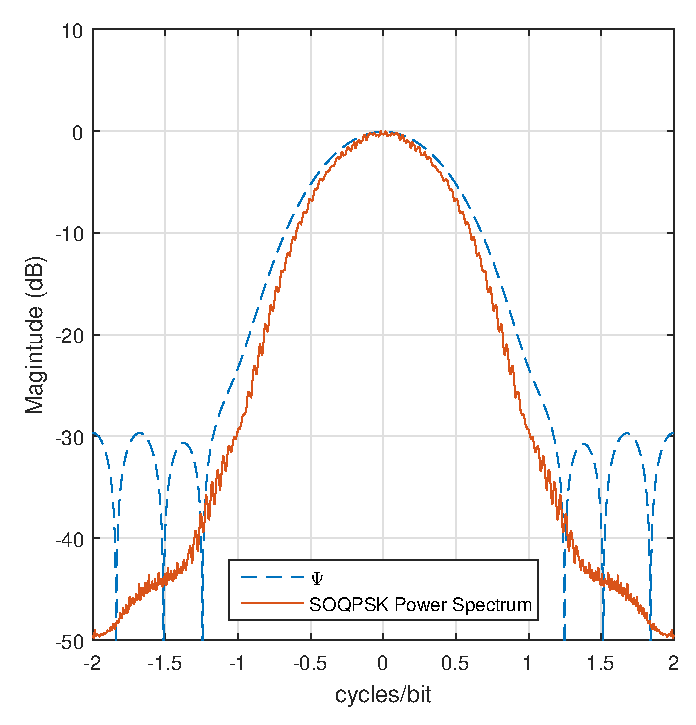
\includegraphics[width=5in]{figures/eq_equations/FDE2_spectrum_PSI.eps}
	\label{fig:SOQPSK_spectrum}
\end{figure}





%%%%%%%%%%%%% begin Bibliography %%%%%%%%%%%%%%%%%
%\phantomsection %Forces a new section prior to setting the bibliography reference point
%\bibliographystyle{IEEEtran}
%\addcontentsline{toc}{chapter}{Bibliography}
%\bibliography{refs}

% Bibliographies are best created and maintained using BibTeX
% To use Bibtex, create a bibliography file, e.g., refs.bib
% The sample file sources.bib shows examples of different
% bibliographic entries.
% The bibliography is created by executing:
%  1.  latex, 2. bibtex, 3. latex, 4. latex
%%%%%%%%%%%%%%%% end Bibliography %%%%%%%%%%%%%%%%%

%Included because WinEdit is RETARDED and it needs it for Gather Purposes:
%input "refs.bib"


% Include appendix sections here:
% each appendix should be a file with a .tex extension and the text
% of the file should begin with \appendix{Appendix Title}, followed
% by the contents of the appendix
%\appendix{Sample Appendix}

\section{Width Based on Page Size Figure Example} \label{sec:appendxia_figure_example}
Here's an example of a figure whose width depends on the width
of the page. You can see if as Figure \ref{fig:appendix_some_pic}.

\begin{figure}[htbp]
  \centering
  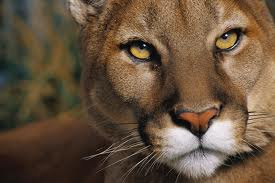
\includegraphics[width=0.45\textwidth]{figures/appendixa/some_pic}
  \caption[Example Width Based on Page Size Figure]{
    This is an example of a figure whose width will be 45\% of the
    width of the page. If you'd like to see a figure with a fixed
    width then you can see it as Figure \ref{fig:intro_stuff} in
    Section \ref{sec:intro_figure_example}. Just FYI, I made this
    figure with PowerPoint and then copied it and pasted it into
    wmf2eps and choose the "Paste EMF" option. It will generate
    a larger file, but it will look a TON better than the
    "Paste WMF" option and the "Paste DIB" option will paste the
    rasterized image that won't scale well at all.}
  \label{fig:appendix_some_pic}
\end{figure}

%End the document
\end{document}
